%=============================================================
%  LA-JSSA : Localization-Aware Joint Spectrum Sensing & Access
%  SINGLE-FILE SOURCE.
%  Build:  pdflatex la_jssa  ->  bibtex la_jssa  ->  pdflatex x2
%  (a self-contained .bbl is also inlined at the bottom; if you keep
%   references.bib next to this file, bibtex will regenerate it.)
%  NOTATION: all symbols are defined in the macro block below and used
%  consistently throughout (the notation-macros convention).
%=============================================================
\documentclass[journal]{IEEEtran}

\usepackage{amsmath,amssymb,amsfonts,amsthm}
\usepackage{mathtools}
\usepackage{bm}
\usepackage{graphicx}
\usepackage{cite}
\usepackage{algorithm}
\usepackage{algpseudocode}
\usepackage{booktabs}
\usepackage{url}
\usepackage[hidelinks]{hyperref}

\newtheorem{theorem}{Theorem}
\newtheorem{lemma}{Lemma}
\newtheorem{proposition}{Proposition}
\newtheorem{corollary}{Corollary}
\newtheorem{assumption}{Assumption}
\newtheorem{definition}{Definition}
\newtheorem{remark}{Remark}
\newtheorem{example}{Example}

%================= NOTATION MACROS (single source of truth) =====
% ============================================================
%  notation_macros.tex
%  SINGLE SOURCE OF TRUTH for all mathematical notation.
%  Every symbol used in the paper is defined here as a macro
%  so that a global change propagates everywhere.
% ============================================================

% ---- generic operators / sets ----
\newcommand{\R}{\mathbb{R}}
\newcommand{\Nat}{\mathbb{N}}
\newcommand{\Prob}{\mathbb{P}}
\newcommand{\E}{\mathbb{E}}
\newcommand{\Ind}{\mathbf{1}}             % indicator function
\newcommand{\defeq}{\triangleq}
\DeclareMathOperator*{\argmax}{arg\,max}
\DeclareMathOperator*{\argmin}{arg\,min}
\DeclareMathOperator{\sgn}{sgn}

% ---- signal / STFT model ----
\newcommand{\rx}{r}                       % received continuous signal r(t)
\newcommand{\sutx}{x}                      % SU transmitted signal
\newcommand{\noise}{w}                     % AWGN
\newcommand{\Npu}{N_{\mathrm{p}}}          % number of PU emissions
\newcommand{\fs}{f_{\mathrm{s}}}           % sampling rate
\newcommand{\Wband}{W}                     % total monitored bandwidth
\newcommand{\fc}{f_{\mathrm{c}}}           % center frequency (sensor)
\newcommand{\STFT}{\mathcal{S}}            % STFT operator
\newcommand{\spec}{\bm{X}}                 % spectrogram (magnitude) matrix
\newcommand{\Nf}{N_f}                      % number of frequency bins
\newcommand{\Nt}{N_t}                      % number of time bins (per frame)
\newcommand{\cell}{(m,n)}                  % a TF cell index (freq m, time n)

% ---- PU emission descriptor (continuous TF box) ----
\newcommand{\boxk}{\bm{b}}                 % a TF box b = (fc, BW, ts, dur)
\newcommand{\bfc}{f}                       % box center frequency
\newcommand{\bBW}{\beta}                   % box bandwidth
\newcommand{\bts}{\tau}                    % box start time
\newcommand{\bdur}{\delta}                 % box duration

% ---- occupancy / belief map ----
\newcommand{\occ}{O}                       % true occupancy O_{m,n} in {0,1}
\newcommand{\bel}{B}                       % belief map B_{m,n} in [0,1]
\newcommand{\belmap}{\bm{B}}               % full belief map matrix
\newcommand{\occmap}{\bm{O}}               % full true occupancy matrix
\newcommand{\Pmd}{P_{\mathrm{md}}}         % cell-level miss-detection prob
\newcommand{\Pfa}{P_{\mathrm{fa}}}         % cell-level false-alarm prob
\newcommand{\thr}{\eta}                    % decision threshold on belief

% ---- access action ----
\newcommand{\act}{\bm{a}}                  % access action (resource block)
\newcommand{\afc}{f^{\mathrm{a}}}          % action center freq
\newcommand{\aBW}{\beta^{\mathrm{a}}}      % action bandwidth
\newcommand{\ats}{\tau^{\mathrm{a}}}       % action start time
\newcommand{\adur}{\delta^{\mathrm{a}}}    % action duration
\newcommand{\pwr}{p}                       % transmit power
\newcommand{\pmax}{p_{\max}}               % power budget
\newcommand{\dmin}{\beta_{\min}}           % minimum bandwidth demand

% ---- POMDP / RL ----
\newcommand{\state}{\bm{s}}                % state
\newcommand{\obs}{\bm{o}}                  % observation
\newcommand{\histlen}{H}                   % history length (ConvLSTM window)
\newcommand{\rew}{r}                       % reward (overloaded w/ rx? use R)
\renewcommand{\rew}{\mathcal{R}}           % reward function
\newcommand{\pol}{\pi}                     % policy
\newcommand{\polopt}{\pi^{\star}}          % optimal policy
\newcommand{\disc}{\gamma}                 % discount factor
\newcommand{\Qfun}{Q}                      % action-value
\newcommand{\Vfun}{V}                      % state-value
\newcommand{\bigT}{T}                      % horizon

% ---- performance metrics ----
\newcommand{\Pcol}{P_{\mathrm{col}}}       % PU collision probability
\newcommand{\Pcolmax}{P_{\mathrm{col}}^{\max}} % collision constraint
\newcommand{\thru}{\mathsf{R}}             % achievable throughput
\newcommand{\thrumax}{\mathsf{R}_{\max}}   % max (oracle) throughput
\newcommand{\util}{U}                      % spectrum utilization
\newcommand{\regret}{\mathrm{Reg}}         % regret

% ---- policy classes (Theorem B) ----
\newcommand{\PIbel}{\Pi_{\mathrm{bel}}}    % belief-state policy class
\newcommand{\PIdis}{\Pi_{\mathrm{disc}}}   % fixed-channel discretized class
\newcommand{\quanterr}{\epsilon_{\mathrm{q}}} % quantization distortion bound

% ---- M1: distributional / CVaR risk-sensitive macros ----
\newcommand{\Zret}{Z}                       % return distribution (random)
\newcommand{\Zcol}{Z_{\mathrm{col}}}        % collision return (random)
\newcommand{\Zthru}{Z_{\mathsf{R}}}         % throughput return (random)
\DeclareMathOperator{\CVaR}{CVaR}
\DeclareMathOperator{\VaR}{VaR}
\newcommand{\cvarlvl}{\alpha}               % CVaR tail level for throughput
\newcommand{\cvarcol}{\beta}                % CVaR tail level for collision
\newcommand{\thrcvar}{\thr^{\star}_{\mathrm{CVaR}}} % CVaR-optimal threshold
\newcommand{\Qinv}{F^{-1}}                   % quantile function

\newcommand{\hidden}{\bm{s}^{\mathrm{h}}}   % hidden state (true occupancy + box params)
\newcommand{\PcolmaxW}{P_{\mathrm{col},W}^{\max}}  % per-window collision budget
\newcommand{\iou}{\mathrm{IoU}}
\newcommand{\eloc}{\varepsilon_{\mathrm{loc}}}
\newcommand{\cmd}{c_{\mathrm{md}}}
\newcommand{\cfa}{c_{\mathrm{fa}}}
\newcommand{\rmd}{r_{\mathrm{md}}}
\newcommand{\rfa}{r_{\mathrm{fa}}}
\newcommand{\fint}{I}
\newcommand{\flo}{f_{\mathrm{lo}}}
\newcommand{\fhi}{f_{\mathrm{hi}}}

\begin{document}

\title{From Time--Frequency Localization to Risk-Sensitive Access:
A Belief-Map Closed Loop for Wideband Cognitive Radio}

\author{Runyi~Zhao
\thanks{Manuscript draft, \today. R.~Zhao is with Xidian University, Xi'an,
China (e-mail: runyizhao@example.edu).}}

\markboth{IEEE Transactions Journal}%
{Zhao: Localization-Aware Joint Spectrum Sensing and Access}

\maketitle

\begin{abstract}
Dynamic spectrum access (DSA) schemes based on deep reinforcement
learning (DRL) almost universally assume that the wideband spectrum is
pre-partitioned into a fixed grid of channels, each in a binary good/bad
state. This assumption breaks down in real wideband environments, where
primary-user (PU) emissions occupy \emph{arbitrary} center frequencies,
bandwidths, and durations---precisely the regime addressed by
time--frequency (TF) localization. We close the loop between the two: the
sensing module outputs a \emph{continuous occupancy belief map} over the TF
plane, which serves directly as the state of the access agent; the agent
selects a TF resource block. We cast the problem as a partially observed
control problem with a learned soft-occupancy observation, and analyze (i) a
propagation bound mapping localization error ($P_{\mathrm{md}},
P_{\mathrm{fa}}$) to PU-collision probability and throughput loss, yielding a
three-way sensing-accuracy/throughput/PU-protection trade-off with a
characterized operating point; (ii) an information-refinement result showing
the belief-state representation is no worse than a coarser fixed-channel one
under a common action space; and (iii) a risk-sensitive, conditional
value-at-risk (CVaR) access formulation whose operating point is provably at
least as conservative as the mean-constrained one. A stylized regret analysis for a tabular surrogate
separates a vanishing learning cost from a policy-independent sensing gap.
Simulations on a continuous-bandwidth, non-grid PU model confirm the
predicted operating point and the tail-risk reduction, and show that access
performance is governed by \emph{frequency}-localization accuracy---which the
analysis ties to access throughput through the localizer's
intersection-over-union (IoU).
\end{abstract}

\begin{IEEEkeywords}
Dynamic spectrum access, spectrum sensing, time--frequency localization,
deep reinforcement learning, partial observation, cognitive radio.
\end{IEEEkeywords}
\section{Introduction}
\label{sec:introduction}

\IEEEPARstart{S}{pectrum} scarcity has become a defining bottleneck for
modern and forthcoming wireless systems. Dynamic spectrum access (DSA),
in which secondary users (SUs) opportunistically reuse spectrum left idle by
primary users (PUs), is widely regarded as a key remedy and underpins
emerging shared-spectrum regimes such as the citizen broadband radio service
(CBRS)~\cite{sohul2015cbrs}. Realizing DSA requires solving two tightly
coupled subproblems: \emph{spectrum sensing}, which estimates what spectrum
is free, and \emph{spectrum access}, which decides how to use it. Because the
quality of sensing directly bounds what access can achieve, and because the
performance after access is the only meaningful measure of whether a sensing
decision was good, a joint treatment of the two is necessary rather than
optional.

Two largely separate research lines have matured around these subproblems.

The first, \emph{time--frequency (TF) localization} (TFL), treats the
wideband spectrogram as an image and applies object detection to output, for
every emission, a bounding box describing its center frequency, bandwidth,
start time, and duration~\cite{prasad2020,li2022hf}. Because the wideband
spectrogram and image object detection are structurally similar, a sequence
of detectors has been adapted to TFL, including region-based and You Only Look
Once (YOLO)-family architectures~\cite{prasad2020,li2022hf}, anchor-free
keypoint detectors that resolve the prior-anchor mismatch caused by the diverse
aspect ratios of radio-frequency (RF) emissions~\cite{zhao2024uav}, and transformer backbones that remain robust
when emissions overlap in the TF plane~\cite{zhao2025trtfl_ssl,
zhang2024spectrumtransformer}. This line has steadily improved how precisely
and robustly a wideband sensor can describe occupancy. Yet it terminates at
sensing: it produces a rich, continuous, often uncertainty-bearing
description of the spectrum and then does nothing with it. The access
decision is left out of scope.

The second line applies \emph{deep reinforcement learning (DRL) to DSA},
learning access---and sometimes sensing---policies under partial
observability~\cite{wang2018,zhong2019,xu2020partial,li2020aggregation,
li2024hmadrl,bokobza2023ddqsa}. Deep $Q$-networks (DQNs)~\cite{wang2018},
actor--critic methods~\cite{zhong2019}, recurrent $Q$-networks for partial
observation~\cite{xu2020partial,hausknecht2015drqn}, and channel-aggregation
schemes~\cite{li2020aggregation} have progressively enlarged the action space
and improved sample efficiency. Almost without exception, however, this line
assumes the wideband spectrum is pre-partitioned into a \emph{fixed grid of
channels}, each summarized by a binary good/bad or idle/busy state.

These two lines are separated by an assumption that is rarely examined. The
DRL-DSA line inherits a fixed channelization in which PU activity is aligned
to grid cells. But real wideband emissions occupy \emph{arbitrary} center
frequencies, bandwidths, and durations---and in shared-spectrum regimes such
as CBRS the center frequency and subchannel division of incumbents change
adaptively with traffic and channel state~\cite{sohul2015cbrs,zhao2025trtfl_ssl}.
This is precisely the regime the TFL line was built to handle. Once occupancy
is not grid-aligned, the ``good/bad channel'' state that DRL-DSA agents
consume is itself a lossy, and sometimes incorrect, summary of the
environment: a single grid cell may straddle the boundary of a PU emission,
forcing the agent either to collide or to abandon usable spectrum. To our
knowledge, no prior work feeds the \emph{continuous, uncertainty-bearing} TF
occupancy estimate produced by a localizer \emph{into} the access decision as
the agent's state, nor analyzes how the localizer's errors propagate to access
performance and PU protection. Closing that loop, and analyzing it, is the
subject of this paper.

We propose \emph{Localization-Aware Joint Spectrum Sensing and Access}
(LA-JSSA), in which the sensing module emits a continuous occupancy
\emph{belief map} over the TF plane that directly serves as the access
agent's state, and the agent selects a continuous TF resource block for
transmission. We further develop a distributional~\cite{dabney2018qrdqn}, risk-sensitive access tier
(D-LA-JSSA) tailored to the belief-state representation. Our contributions
are:
\begin{enumerate}
\item \textbf{A belief-map closed loop.} We formulate joint sensing and
access as a partially observed control problem whose state is the continuous TF occupancy
posterior rather than a fixed-channel vector
(Section~\ref{sec:system_model}), realized by a two-timescale architecture
that couples a supervised TFL sensing tier to a reinforcement-learned access
tier without unstable end-to-end training (Section~\ref{sec:framework}).
\item \textbf{Error-propagation analysis and a three-way trade-off.} We map
cell-level localization error ($\Pmd,\Pfa$) to PU-collision probability and
SU throughput, yielding a sensing-accuracy/throughput/PU-protection
trade-off with a characterized optimal belief threshold $\thr^\star$
(Theorem~\ref{thm:tradeoff}), and a linear bound on the price of imperfect
localization (Corollary~\ref{cor:price}).
\item \textbf{Risk-sensitive access via a distributional critic.} We cast
access as a \emph{distributional} reinforcement-learning (RL)
problem~\cite{dabney2018qrdqn,ma2020dsac} with a tail-risk conditional
value-at-risk (CVaR) constraint on PU collision, and show its operating point is at least as
conservative as the mean-constrained one, with a first-order estimate of the
conservativeness margin (Theorem~\ref{thm:cvar},
Corollary~\ref{cor:cvargap}).
\item \textbf{Information refinement and a stylized regret analysis.} We show
the belief-state policy class is no worse than any coarser fixed-channel
representation under a common action space
(Proposition~\ref{thm:sufficiency}), with a strict gap on a misaligned
instance (Example~\ref{ex:strictgap}); and, for a tractable tabular
surrogate, we separate the regret into a vanishing learning term and a
policy-independent sensing gap (Proposition~\ref{thm:regret}). The latter is a
stylized analysis, not a guarantee for the deep agent.
\item \textbf{Validation.} Simulations on a continuous-bandwidth, non-grid
PU model confirm the predicted operating point and the tail-risk reduction,
validate the full sensing-error propagation chain end to end, and show the
belief-map advantage is monotone in representation richness and robust across
traffic, geometry, and SNR regimes (Section~\ref{sec:simulation}).
\end{enumerate}
The remainder of the paper is organized as follows.
Section~\ref{sec:related_work} reviews related work,
Section~\ref{sec:system_model} formulates the model,
Section~\ref{sec:framework} presents LA-JSSA,
Section~\ref{sec:theory} develops the theory,
Section~\ref{sec:simulation} reports experiments, and
Section~\ref{sec:conclusion} concludes.


\section{Related Work}
\label{sec:related_work}

We organize prior work into three strands---TF localization, DRL-based
access, and joint sensing-and-access---and state, for each, the precise
distinction from LA-JSSA.

\subsection{Time--Frequency Localization for Wideband Sensing}
Classical spectrum sensing---energy, matched-filter, cyclostationary, and
covariance-based detectors---is surveyed
in~\cite{yucek2009survey,axell2012spectrum,arjoune2019comprehensive}.
Scanning-based wideband sensing divides the spectrum into subbands according
to a known channelization and applies narrowband detection in each
subband~\cite{wang2018}. In shared bands such as CBRS and the industrial,
scientific, and medical (ISM) bands, however, the
center frequency and subchannel division of incumbents change adaptively with
service demand and channel state, so methods that presuppose a fixed
channelization fail~\cite{sohul2015cbrs}. Deep learning has since been applied
to over-the-air signal classification~\cite{oshea2018over,oshea2021dataset}
and wideband signal detection~\cite{vo2020wideband}. TFL was introduced
precisely to remove the fixed-channelization assumption: by casting the
magnitude spectrogram as an image and applying object detection, a detector
can simultaneously estimate the time and frequency support of every
emission~\cite{prasad2020,prasad2021spectrum}.

A detector lineage has followed. Downscaled Faster R-CNN (region-based
convolutional neural network) and YOLO-family
detectors~\cite{redmon2018yolov3} were first adapted to signal TFL~\cite{prasad2020,li2022hf}. The
diverse aspect ratios of RF emissions cause a prior-anchor mismatch in
anchor-based detectors; anchor-free keypoint detectors with tailored matching
were proposed to resolve it and to classify multiple co-existing
emitters~\cite{zhao2024uav}. When emissions overlap in the TF plane---as they
do under concurrent spectrum reuse---convolutional backbones lose
discriminative features; transformer backbones that exploit TF correlation,
optionally with masked-autoencoder pre-training~\cite{he2022mae} to overcome label scarcity,
achieve state-of-the-art robustness~\cite{zhao2025trtfl_ssl,
zhang2024spectrumtransformer,he2022mae}. Collectively, this line has made the
occupancy description ever more precise and robust. \emph{Our distinction:}
every one of these works terminates at sensing, emitting boxes (or, after
non-maximum suppression (NMS), hard decisions) that are never coupled to an access
policy. We instead retain the detector's \emph{soft} output as a belief state
and close the loop to access.

\subsection{DRL for Dynamic Spectrum Access}
DRL-based DSA learns channel-selection policies under partial observability,
building on the DQN~\cite{mnih2015human} and modern
policy-gradient methods such as proximal policy optimization
(PPO)~\cite{schulman2017ppo} and soft actor--critic
(SAC)~\cite{haarnoja2018sac}. DQNs were applied to
multichannel access with correlated channel occupancy~\cite{wang2018};
actor--critic frameworks improved performance in large action
spaces~\cite{zhong2019}; recurrent $Q$-networks addressed partial observation
by summarizing observation histories~\cite{xu2020partial,hausknecht2015drqn,
xu2021deep}; reservoir-computing and multi-user variants targeted distributed
access~\cite{chang2019distributive,naparstek2018deep}; upper-confidence-bound
(UCB)-style exploration was used in cooperative sensing~\cite{zhang2019deep}; and
spectrum-aggregation schemes let an SU combine several idle channels to meet a
bandwidth demand~\cite{li2020aggregation}. Related efforts apply DRL to joint
channel and power control~\cite{tan2020deep} and to cognitive radio sensor
networks~\cite{lin2019deep}. These methods share a structural premise: the
state is defined on a \emph{fixed channel grid} with binary occupancy, and the
action selects one or more whole grid channels. \emph{Our distinction:} our
state is a continuous TF belief map with no grid, our action is a continuous
resource block, and---uniquely---we analyze how sensing error propagates into
this continuous access problem.

Safety and risk in RL are also relevant to our CVaR access constraint.
Constrained Markov decision processes (MDPs)~\cite{altman1999constrained} and their deep solvers
(constrained policy optimization~\cite{achiam2017cpo}, reward-constrained
policy optimization~\cite{tessler2019reward}) enforce expected-cost limits,
while percentile- and CVaR-based criteria~\cite{chow2017risk,rockafellar2000cvar}
and distributional RL~\cite{bellemare2017distributional,dabney2018qrdqn,
ma2020dsac} target the tail. We adopt a distributional critic with a CVaR
collision constraint and connect its operating point to the sensing error.

\subsection{Joint Sensing-and-Access}
Closest to us are works that jointly design sensing and access. The classical
sensing--throughput trade-off optimizes the sensing \emph{duration} and an
energy threshold for a \emph{single} channel, trading detection against
false alarm along the time axis~\cite{liang2008sensing}; it does not address
a two-dimensional continuous TF plane or a learned localizer. Among learning
approaches, double deep $Q$-learning has been used to learn sensing and
access policies jointly, but in a \emph{narrowband, single-channel} setting
without TF localization or continuous boxes~\cite{bokobza2023ddqsa}.
Hierarchical multi-agent DRL jointly selects a sensing window and power
allocation, yet its state remains discrete band occupancy on a fixed
grid~\cite{li2024hmadrl}. Cooperative sensing-and-access for the industrial
Internet of Things (IoT) integrates the two via optimization rather than
learning~\cite{liu2023ciiot}.
Interference-temperature-constrained DSA formalizes PU protection but again
on predefined channels~\cite{xing2007dsa}. \emph{Our distinction:} LA-JSSA
operates on a two-dimensional continuous TF plane, drives access directly
from a learned occupancy belief map, analyzes the resulting
sensing-accuracy/throughput/PU-protection trade-off as a function of
localization error, and protects the PU through a tail-risk (CVaR) constraint
rather than a mean constraint---a regime, to our knowledge, not previously
treated.


\section{System Model and Problem Formulation}
\label{sec:system_model}

We consider a single SU opportunistically accessing a
wideband spectrum of bandwidth $\Wband$ centered at $\fc$, which is
shared by an \emph{unknown and time-varying} number of PU
emissions. Such a setting arises in shared bands such as CBRS, where
incumbents select center frequencies and bandwidths adaptively rather than on
a fixed channel grid~\cite{sohul2015cbrs,xing2007dsa}. Unlike the
fixed-channel models prevalent in the DRL-based DSA literature, we make
\emph{no} assumption that PU activity is aligned to a predefined channel
grid: each PU emission occupies an arbitrary center frequency, bandwidth,
start time, and duration, exactly the regime targeted by TF
localization~\cite{prasad2020,zhao2025trtfl_ssl}. The notation introduced
below is summarized in Table~\ref{tab:notation}.

\begin{table}[t]
\centering
\caption{Summary of Notation}
\label{tab:notation}
\begin{tabular}{ll}
\toprule
Symbol & Meaning \\
\midrule
$\spec\in\R_{\ge0}^{\Nf\times\Nt}$ & Magnitude spectrogram (frame) \\
$\cell$ & TF cell (freq.\ bin $m$, time bin $n$) \\
$\boxk_k=(\bfc_k,\bBW_k,\bts_k,\bdur_k)$ & $k$-th PU emission box \\
$\occmap\in\{0,1\}^{\Nf\times\Nt}$ & True occupancy map \\
$\belmap\in[0,1]^{\Nf\times\Nt}$ & Estimated occupancy belief map \\
$\Pmd,\Pfa$ & Cell-level miss/false-alarm prob.\ \\
$\thr$ & Belief decision threshold \\
$\act=(\afc,\aBW,\ats,\adur,\pwr)$ & SU access action (resource block) \\
$\dmin,\pmax$ & Min.\ bandwidth demand, power budget \\
$\state_t,\obs_t$ & Access state, observation \\
$\rew,\disc,\pol$ & Reward, discount, policy \\
$\Pcol,\Pcolmax$ & PU collision prob.\ and its cap \\
$\thru,\thrumax$ & Achievable / oracle throughput \\
\bottomrule
\end{tabular}
\end{table}

\subsection{Wideband Signal and Spectrogram Model}
\label{subsec:signal}
The complex baseband signal observed by the wideband sensor over one frame
is
\begin{equation}
\rx(t) \;=\; \sum_{k=1}^{\Npu} c_k\!\left(\sutx_k(t)\right) \;+\; \noise(t),
\qquad 0 \le t < \bigT_{\mathrm{f}},
\label{eq:rx}
\end{equation}
where $\sutx_k(t)$ is the $k$-th PU emission, $c_k(\cdot)$ denotes the
corresponding channel (carrying carrier offset, bandwidth-limiting, and
fading), $\noise(t)$ is additive white Gaussian noise, $\Npu$ is the
(random, unknown) number of active emissions in the frame, and
$\bigT_{\mathrm{f}}$ is the frame length. The signal is sampled at rate
$\fs \ge \Wband$.

Applying the short-time Fourier transform (STFT) operator $\STFT$ yields a
single-resolution TF representation; we work with the
magnitude spectrogram
\begin{equation}
\spec \;=\; \bigl|\STFT\{\rx\}\bigr| \;\in\; \R_{\ge 0}^{\,\Nf \times \Nt},
\label{eq:stft}
\end{equation}
discretized into $\Nf$ frequency bins and $\Nt$ time bins. We index an
individual TF \emph{cell} by $\cell$, $m\in\{1,\dots,\Nf\}$,
$n\in\{1,\dots,\Nt\}$. The STFT is preferred over variable-resolution
transforms (the continuous wavelet transform or constant-$Q$ transform)
because spectrum monitoring weights all frequencies equally~\cite{prasad2020}.

\subsection{Continuous Occupancy Representation}
\label{subsec:occupancy}
Each PU emission $k$ is described by a continuous TF \emph{box}
\begin{equation}
\boxk_k \;=\; \bigl(\bfc_k,\, \bBW_k,\, \bts_k,\, \bdur_k\bigr),
\label{eq:box}
\end{equation}
i.e.,\ center frequency, bandwidth, start time, and duration. The box maps to
a region $\mathcal{B}_k \subset \{1,\dots,\Nf\}\times\{1,\dots,\Nt\}$ of the
discretized TF plane. The \emph{true occupancy map} is the binary matrix
$\occmap\in\{0,1\}^{\Nf\times\Nt}$ with
\begin{equation}
\occ_{m,n} \;=\;
\Ind\!\Bigl\{\, \cell \in \textstyle\bigcup_{k=1}^{\Npu}\mathcal{B}_k \,\Bigr\},
\label{eq:occupancy}
\end{equation}
where $\occ_{m,n}=1$ marks a cell occupied by at least one PU. Crucially,
$\occmap$ is \emph{not} block-structured along a fixed channelization;
recovering it is exactly the TF-localization problem.

We clarify the sense in which the model is ``grid-free.'' The PU
\emph{emission parameters} \eqref{eq:box} are continuous; they are mapped to
an occupancy map discretized at the \emph{sensing resolution} $\Nf\times\Nt$
of the STFT. The point is not the absence of any discretization---a finite
spectrogram is necessarily discretized---but the absence of a fixed
\emph{communication channel grid} to which PU activity is assumed aligned.
Emissions may occupy arbitrary cells at sensing resolution, straddling any
notional channel boundary, which is precisely what defeats fixed-channel DSA
models and motivates the localization-driven treatment.

\subsection{Sensing Model: From Spectrogram to Belief Map}
\label{subsec:sensing}
The sensing module is a learned mapping $\phi_{\mathrm{sen}}$ that estimates,
for each cell, the posterior probability of PU occupancy:
\begin{equation}
\belmap = \phi_{\mathrm{sen}}(\spec) \in [0,1]^{\Nf\times\Nt},
\quad
\bel_{m,n} \approx \Prob(\occ_{m,n}{=}1 \mid \spec).
\label{eq:belief}
\end{equation}
Concretely, $\bel_{m,n}$ is the \emph{detection confidence} of the
time--frequency localizer rasterized onto the cell grid: each estimated
emission box carries a confidence score, and $\bel_{m,n}$ is the (edge-feathered)
score of the box covering cell $(m,n)$, or a low background value where no box
is predicted. We deliberately retain this \emph{soft} confidence $\belmap$
rather than applying NMS to obtain hard boxes; this
preserves the sensing uncertainty that the access stage will exploit
(cf.\ Section~\ref{sec:framework}). The reliability of $\phi_{\mathrm{sen}}$
is characterized at the cell level by the miss-detection and false-alarm
probabilities
\begin{align}
\Pmd &\defeq \Prob\!\left(\bel_{m,n} < \thr \;\middle|\; \occ_{m,n}=1\right),
\label{eq:pmd}\\
\Pfa &\defeq \Prob\!\left(\bel_{m,n} \ge \thr \;\middle|\; \occ_{m,n}=0\right),
\label{eq:pfa}
\end{align}
where $\thr\in[0,1]$ is a decision threshold applied to the localizer's
confidence $\bel_{m,n}$. Two distinct factors shape $(\Pmd,\Pfa)$: the
\emph{confidence threshold} $\thr$ (where we cut the soft score) and the
\emph{geometric accuracy} of the box (how well its frequency support matches
the true emission, quantified later by the intersection-over-union (IoU)
error $\eloc$). The
operating-point analysis of Theorem~\ref{thm:tradeoff} optimizes over $\thr$,
while the localization-error model of Assumption~\ref{as:localization}
captures the geometric contribution; their separation is made explicit in the
bound \eqref{eq:loc_to_cell}. Both $\Pmd$ and $\Pfa$ are functions of $\thr$;
this dependence is the lever in the trade-off of
Theorem~\ref{thm:tradeoff} (Section~\ref{sec:theory}).

\subsection{Access Model: Continuous Resource Selection}
\label{subsec:access}
The SU operates a sense-then-access frame: the sensing phase estimates the
occupied frequency ranges, and the access phase of the \emph{same} frame
transmits in the ranges it deems idle. Because both phases share the frame,
temporal alignment is given, and the access decision turns on \emph{which
frequencies} are free---making frequency-localization accuracy, rather than
temporal extent, the quantity that governs access performance (formalized in
Section~\ref{sec:theory}). At each frame the SU chooses a continuous TF
resource block together with a transmit power level,
\begin{equation}
\act \;=\; \bigl(\afc,\, \aBW,\, \ats,\, \adur,\, \pwr\bigr),
\label{eq:action}
\end{equation}
subject to the bandwidth demand, power, and PU-protection constraints
\begin{equation}
\aBW \ge \dmin, \quad 0 \le \pwr \le \pmax, \quad
\Prob(\text{collision}) \le \Pcolmax .
\label{eq:constraints}
\end{equation}
A \emph{collision} occurs when the SU block overlaps an occupied cell:
\begin{equation}
\mathrm{Col}(\act) \defeq
\Ind\!\Bigl\{\, \exists\,\cell \in \mathcal{A}(\act):\; \occ_{m,n}=1 \,\Bigr\},
\label{eq:collision}
\end{equation}
where $\mathcal{A}(\act)$ is the set of TF cells covered by action $\act$.
Transmission succeeds (yielding an acknowledgment, ACK) iff $\mathrm{Col}(\act)=0$ and the
allocated bandwidth meets the demand.

\subsection{Partially Observed Control Formulation}
\label{subsec:pomdp}
The SU never observes the true occupancy $\occmap$ directly; it observes only
the wideband spectrogram $\spec_t$ and, after transmitting, a one-bit
ACK or negative-acknowledgment (NACK). The control problem is therefore
partially observed. We make the
roles explicit to avoid conflating the detector output with a Bayesian
belief.

\paragraph*{Hidden state} The hidden state is the true PU occupancy together
with the underlying emission parameters,
$\hidden_t=\bigl(\occmap_t,\{\boxk\}\bigr)$, evolving as a
(piecewise-stationary) Markov process.

\paragraph*{Observation} The raw observation is the spectrogram $\spec_t$ and
the ACK/NACK $\mathrm{ACK}_t\in\{0,1\}$. The sensing tier maps $\spec_t$ to
the per-cell soft occupancy estimate $\belmap_t\in[0,1]^{\Nf\times\Nt}$ of
\eqref{eq:belief}. We stress that $\belmap_t$ is a learned \emph{soft
occupancy observation feature}, not the exact Bayesian posterior
$\Prob(\hidden_t\mid\text{history})$; it plays the role of an
\emph{approximate sufficient statistic} of the observation history for the
access decision.

\paragraph*{Access state} The access policy acts on the recent history of
this feature,
\begin{equation}
\state_t \;=\; \bigl(\belmap_{t-\histlen+1},\dots,\belmap_{t}\bigr)
\;\in\; [0,1]^{\histlen \times \Nf \times \Nt},
\label{eq:state}
\end{equation}
stacked over a short window to capture temporal correlation of PU activity.
This continuous, uncertainty-bearing state is the central departure from
prior DRL-DSA work, whose state is a binary fixed-channel occupancy vector.
Because $\belmap$ approximates rather than equals the exact posterior, the
formulation is a \emph{partially observed control problem with a learned
observation feature} rather than a belief-MDP in the strict Bayesian sense;
the theoretical claims of Section~\ref{sec:theory} are stated against this
representation and do not presume exact belief recursion.

\paragraph*{Reward} We use an uncertainty-aware reward that rewards
throughput, penalizes PU collisions, and discourages transmitting into
low-confidence regions:
\begin{equation}
\rew(\state_t,\act_t) \;=\;
\underbrace{\thru(\act_t)}_{\text{throughput}}
\;-\; \lambda_{\mathrm{c}}\,\mathrm{Col}(\act_t)
\;-\; \lambda_{\mathrm{u}}\,\mathcal{U}\!\left(\belmap_t,\act_t\right),
\label{eq:reward}
\end{equation}
where $\mathcal{U}(\cdot)$ measures the residual occupancy uncertainty over
the chosen block and $\lambda_{\mathrm{c}},\lambda_{\mathrm{u}}\ge 0$ are
weights. The connection of the $\lambda_{\mathrm{u}}$ term to a
risk-sensitive objective is discussed in Section~\ref{sec:framework}.

\paragraph*{Objective} The SU seeks a policy
$\pol:\mathcal{S}\to\mathcal{A}$ maximizing the expected discounted return
subject to the PU-protection constraint,
\begin{equation}
\begin{aligned}
\polopt = \argmax_{\pol}\;
&\E_{\pol}\!\left[\sum_{t=0}^{\infty}\disc^{t}
\rew(\state_t,\act_t)\right]\\[-1pt]
\text{s.t.}\quad
&\E_{\pol}\!\left[\mathrm{Col}(\act_t)\right] \le \Pcolmax .
\end{aligned}
\label{eq:objective}
\end{equation}

\begin{remark}
Setting $\belmap$ to a binary fixed-channel vector and restricting $\act$ to
a single grid channel recovers the standard formulation of
\cite{wang2018,zhong2019} as a special case. Proposition~\ref{thm:sufficiency}
formalizes that this restriction can be strictly suboptimal under grid misalignment.
\end{remark}

\section{The LA-JSSA Framework}
\label{sec:framework}

We now describe the two-timescale architecture that realizes the partially
observed control problem of Section~\ref{sec:system_model}. The design
separates a slowly-adapted supervised \emph{sensing tier}, which produces the
occupancy belief map $\belmap$, from a fast \emph{access tier} that learns the
policy $\pol$ by reinforcement~\cite{sutton2018rl}. Fig.~\ref{fig:arch} shows how the two tiers
close the sensing--access loop: the data flow
$\rx\to\spec\to\belmap\to\state\to\act$ feeds forward through the network,
and ACK/collision feedback from the environment returns to both the localizer
and the risk-constrained critic.

\begin{figure*}[t]
\centering
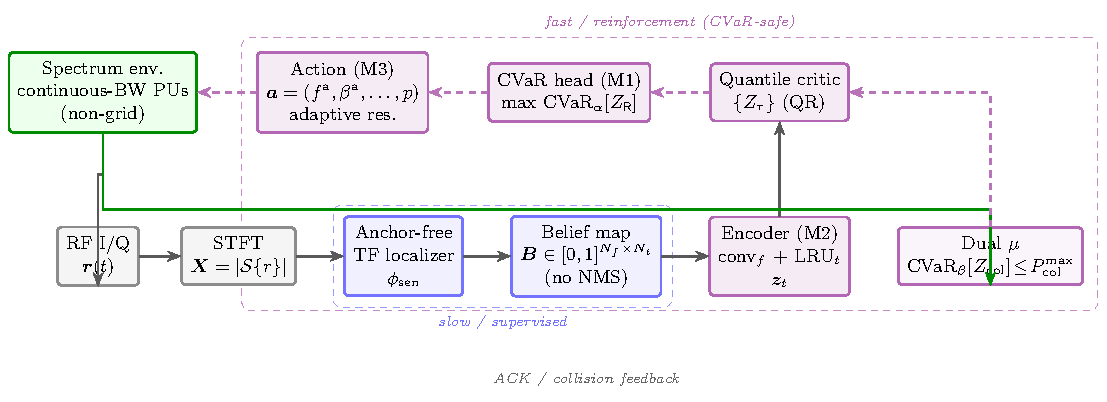
\includegraphics[width=0.95\textwidth]{figures/fig_arch.pdf}
\caption{The D-LA-JSSA two-timescale architecture. \emph{Bottom (slow,
supervised):} wideband in-phase/quadrature (I/Q) data are transformed to a spectrogram and passed to an
anchor-free TF localizer $\phi_{\mathrm{sen}}$ that emits a soft occupancy
belief map $\belmap$ (no NMS), encoded across time by a conv$_f$\,+\,LRU$_t$
encoder (M2). \emph{Top (fast, reinforcement):} a quantile critic feeds a
CVaR head (M1) and an adaptive-resolution action head (M3); a dual-ascent
multiplier enforces the CVaR collision constraint from ACK/collision
feedback. The environment of continuous-bandwidth, non-grid-aligned PUs
closes the loop.}
\label{fig:arch}
\end{figure*}

\subsection{Two-Timescale Rationale}
\label{subsec:twotimescale}
Joint end-to-end training of a detector and an RL agent is notoriously
unstable: the non-stationary reward signal corrupts the supervised gradient
of the detector, while a drifting detector keeps the RL state distribution
non-stationary. We therefore decouple the two. The sensing tier
$\phi_{\mathrm{sen}}$ is trained offline (or slowly online) on labeled
spectrograms with a supervised objective, so that the cell-level error rates
$\Pmd(\thr),\Pfa(\thr)$ of Assumption~\ref{as:cellerror} are stable; the
access tier then learns against an approximately stationary observation
channel. This mirrors the decoupled offline/online structure that is known
to accelerate partially observed Markov decision process (POMDP) learning
when the observation model is fixed.

\subsection{Sensing Tier: Belief-Map Generation}
\label{subsec:sensing_tier}
The sensing tier maps a spectrogram frame to the per-cell occupancy
posterior \eqref{eq:belief}. Because PU emissions have widely varying
time--frequency aspect ratios, we adopt an \emph{anchor-free} detector
(center/extent regression over the TF plane) rather than an anchor-based
region proposal network, which couples poorly to continuous, arbitrary
bandwidths~\cite{zhao2024uav}; when emissions overlap, a transformer backbone
that exploits TF correlation further improves
robustness~\cite{zhao2025trtfl_ssl}. The key departure from prior
TF-localization work is that we do \emph{not} apply NMS
to collapse the heatmap into hard boxes; instead the soft per-cell confidence
is retained as the belief map $\belmap\in[0,1]^{\Nf\times\Nt}$. This
preserves exactly the uncertainty that Theorem~\ref{thm:tradeoff} and the
reward \eqref{eq:reward} consume.

\begin{remark}[Design insight]
Discarding the soft confidence (the conventional detector output) is
information-lossy in the precise sense of Proposition~\ref{thm:sufficiency}: a
hard-box state is a deterministic coarsening of $\belmap$. The belief map is
an informative representation for the downstream access decision.
\end{remark}

\subsection{State Encoding Across Time (M2)}
\label{subsec:state_encoding}
To capture temporal correlation of PU activity under partial observability,
the access state \eqref{eq:state} stacks the most recent $\histlen$ belief
maps. The belief map is a two-dimensional TF object, so we encode it with a
\emph{factored} encoder: a convolution along the frequency axis captures the
spatial shape of emissions (their TF extent), while a point-wise linear
recurrent unit (LRU) along the time axis captures the long-range correlation
of PU on/off dynamics, producing a compact latent state
$\bm{z}_t = \mathrm{Enc}(\state_t)$. We adopt an LRU rather than a long
short-term memory (LSTM) network or a Transformer because recent evidence
shows point-wise recurrent state-space
models outperform attention on partially observable RL while remaining
parallelizable and lightweight~\cite{lu2024rethinking,morad2025cae}. The
recurrent encoding plays the role of the belief-update / sufficient-statistic
recursion of a POMDP. We ablate this choice (LRU vs.\ convolutional LSTM,
ConvLSTM) in Section~\ref{sec:simulation}.

\subsection{Access Tier: Continuous Resource Selection}
\label{subsec:access_tier}
The access tier maps the latent state to the resource-block action
\eqref{eq:action}. We consider two instantiations:
\begin{itemize}
\item a value-based agent over a discretized action grid (DQN~\cite{hausknecht2015drqn}
on $\bm{z}_t$), suitable when the TF action set is coarsely quantized; and
\item a continuous-control agent (deep deterministic policy gradient,
DDPG~\cite{lillicrap2016ddpg}) that
outputs $(\afc,\aBW,\ats,\adur,\pwr)$ directly, suitable for fine-grained
continuous resource selection.
\end{itemize}
Both optimize the constrained objective \eqref{eq:objective}; the
PU-protection constraint is enforced via a Lagrangian penalty whose
multiplier tracks the running collision rate against $\Pcolmax$.

\subsection{Distributional Safe Access (M1)}
\label{subsec:dist_rl}
Standard value-based agents learn only the expected return $\E[\Zret]$, which
discards exactly the information the belief map carries: the dispersion of
outcomes induced by occupancy uncertainty. We instead learn the full return
\emph{distribution} via a quantile critic, maintaining quantile estimates of
the throughput return $\Zthru$ and, separately, of the collision return
$\Zcol$. Two consequences follow.

First, the access objective becomes \emph{risk-sensitive}: rather than
$\max\E[\Zthru]$ we maximize a tail-aware utility
$\CVaR_{\cvarlvl}[\Zthru]$~\cite{rockafellar2000cvar}, which protects against rare low-throughput
episodes. Second, and more importantly for PU protection, the constraint is
imposed on the \emph{tail} of the collision-window return $\Zcol^{W}$ of
\eqref{eq:collision_window},
\begin{equation}
\max_{\pol}\;\CVaR_{\cvarlvl}\!\left[\Zthru\right]
\quad\text{s.t.}\quad
\CVaR_{\cvarcol}\!\left[\Zcol^{W}\right]\le\PcolmaxW,
\label{eq:cvar_objective}
\end{equation}
which is the formulation analyzed in Theorem~\ref{thm:cvar}. The CVaR terms
are estimated from the learned quantiles and the constraint is enforced by
dual ascent on a multiplier $\mu$ as in Algorithm~\ref{alg:lajssa}, with the
running windowed collision-CVaR estimate in place of the mean. By
Theorem~\ref{thm:cvar} the resulting operating point is at least as
conservative as the mean-constrained one, by a margin that vanishes as the
localizer sharpens---tying the method back to the value of TF localization.

\begin{remark}[Adaptive action resolution (M3)]
\label{rem:m3}
The quantile critic also exposes per-region uncertainty, which we use to make
the action resolution adaptive: in high-confidence idle regions the agent may
select a coarse, wide resource block, whereas near low-confidence boundaries
it is restricted to fine blocks. This couples the action granularity to the
belief entropy and is evaluated as an ablation in
Section~\ref{sec:simulation}.
\end{remark}

\subsection{Uncertainty-Aware Reward and Risk Sensitivity}
\label{subsec:reward_shaping}
The uncertainty term $\mathcal{U}(\belmap_t,\act_t)$ in the reward
\eqref{eq:reward} penalizes transmitting into TF cells whose occupancy
posterior is close to the undecided region. The following remark gives the
risk-sensitive reading of this penalty; it is an approximate justification,
not a strict equivalence.

\begin{remark}[Uncertainty penalty as a risk proxy]
\label{prop:risk}
Take $\mathcal{U}(\belmap_t,\act_t)=\sum_{\cell\in\mathcal{A}(\act_t)}
\bel_{m,n}(1-\bel_{m,n})$, the summed Bernoulli variance of occupancy over
the accessed cells. \emph{If} cell successes are conditionally independent
given $\belmap_t$ and the block throughput is linear in the per-cell
successes, then the conditional throughput variance is proportional to
$\mathcal{U}$, so $\E[\thru]-\lambda_{\mathrm{u}}\mathcal{U}$ approximates the
mean--variance criterion
$\E[\thru]-\tfrac{\lambda_{\mathrm{u}}}{2}\mathrm{Var}[\thru\mid\belmap_t]$
to second order, with $\lambda_{\mathrm{u}}$ playing the role of a
risk-aversion coefficient. Outside these conditions---correlated cells or
nonlinear reward---$\mathcal{U}$ should be read as an \emph{uncertainty
regularizer / risk proxy} rather than an exact variance, since it penalizes
undecided occupancy rather than interference variance directly.
\end{remark}

\noindent Read this way, the belief-map design is not ad hoc: the
uncertainty penalty steers the agent away from low-confidence cells, which
under the stated conditions coincides with risk-averse behavior. The full
procedure is summarized in Algorithm~\ref{alg:lajssa}.

\begin{algorithm}[t]
\caption{LA-JSSA training (one episode)}
\label{alg:lajssa}
\begin{algorithmic}[1]
\State \textbf{Input:} sensing net $\phi_{\mathrm{sen}}$ (pretrained),
threshold $\thr$, weights $\lambda_{\mathrm{c}},\lambda_{\mathrm{u}}$,
Lagrange multiplier $\mu$
\For{each frame $t$}
  \State acquire $\rx_t$; form spectrogram $\spec_t$ via \eqref{eq:stft}
  \State $\belmap_t \gets \phi_{\mathrm{sen}}(\spec_t)$
         \Comment{soft belief map, no NMS}
  \State $\state_t \gets (\belmap_{t-\histlen+1},\dots,\belmap_t)$;
         $\bm{z}_t \gets \mathrm{Enc}(\state_t)$
  \State select action $\act_t \sim \pol(\cdot\mid\bm{z}_t)$
         (DQN or DDPG head)
  \State transmit; observe ACK $\obs_t$ and collision indicator
  \State $r_t \gets \thru(\act_t) - \lambda_{\mathrm{c}}\mathrm{Col}(\act_t)
         - \lambda_{\mathrm{u}}\mathcal{U}(\belmap_t,\act_t)
         - \mu\,(\mathrm{Col}(\act_t)-\Pcolmax)$
  \State store $(\bm{z}_t,\act_t,r_t,\bm{z}_{t+1})$; update $\pol$
  \State $\mu \gets [\mu + \alpha_\mu(\widehat{\Pcol}-\Pcolmax)]_+$
         \Comment{dual ascent}
\EndFor
\end{algorithmic}
\end{algorithm}

\section{Theoretical Analysis}
\label{sec:theory}

This section analyzes LA-JSSA. Because a single tractable theorem cannot
simultaneously capture the learned detector, the continuous control, and the
finite-time learning dynamics, we analyze the system through a deliberate
\emph{hierarchy of abstractions}---true system (Sec.~\ref{sec:system_model})
$\to$ belief map (Sec.~\ref{sec:framework}) $\to$ fixed-policy evaluation
(Thms.~\ref{thm:tradeoff},~\ref{thm:cvar}) $\to$ tabular surrogate
(Prop.~\ref{thm:regret})---each tier exposing one structural property while
holding the others fixed. The results answer three \emph{distinct} questions
about the same system, and we state up front what each does and does
\emph{not} claim:
\begin{itemize}
\item \textbf{Operating-point analysis} (Theorems~\ref{thm:tradeoff},
\ref{thm:cvar}): a \emph{fixed-policy evaluation} of how the belief threshold
$\thr$---for a fixed action geometry---trades sensing error against
throughput and PU protection, under the mean and the CVaR constraint. These
characterize a static operating point; they are not statements about the
learning process.
\item \textbf{Representation analysis} (Proposition~\ref{thm:sufficiency}):
an information-theoretic comparison of the belief-map state against a coarser
fixed-channel state \emph{under a common action space}. It concerns what is
\emph{representable}, not how it is learned.
\item \textbf{Learning analysis} (Proposition~\ref{thm:regret}): a finite-time
regret bound for a \emph{tabular surrogate} of the access problem. It gives
qualitative insight into the structure of the learning cost; it is
\emph{not} a guarantee for the deep agent of Section~\ref{sec:framework},
which serves as a heuristic solver of the surrogate.
\end{itemize}
We make no claim that the deep RL algorithm inherits these guarantees; the
theory characterizes the surrogate hierarchy, and the experiments
(Section~\ref{sec:simulation}) test whether the predicted \emph{qualitative}
structure carries over to the deep agent.

\begin{remark}[Relation to classical sensing--throughput trade-off]
The classical sensing--throughput trade-off \cite{liang2008sensing} optimizes
the \emph{sensing duration} and an energy threshold for a \emph{single}
channel along the time axis. Theorem~\ref{thm:tradeoff} differs in kind: the
lever is the belief threshold $\thr$ on a \emph{two-dimensional} continuous
TF occupancy estimate, coupling the localization error of a learned detector
to the \emph{access} reward through the collision event
\eqref{eq:collision}.
\end{remark}

\subsection{Assumptions}
\label{subsec:assumptions}

The access stage consumes the output of a \emph{time--frequency localizer},
not a per-channel energy detector. A key structural feature of the
sense-then-access frame simplifies what matters: within one frame, the
sensing phase estimates which \emph{frequency} ranges are unoccupied, and the
access phase of the \emph{same} frame reuses those ranges. The temporal
support of an emission is thus fixed by the frame boundary and given to both
phases; it is the \emph{frequency} extent of each emission that the localizer
must pin down, since a frequency-localization error is what causes the access
phase to either collide (under-estimated occupancy) or waste spectrum
(over-estimated occupancy). We therefore measure localization accuracy by the
\emph{frequency-interval} overlap and relate it to the cell-level error that
drives the access analysis, so that $\Pmd,\Pfa$ are \emph{derived} from
localization quality rather than postulated.

\begin{assumption}[Frequency-localization error model]
\label{as:localization}
For each true PU emission, let its occupied frequency interval in a frame be
$\fint_k=[\flo^{k},\fhi^{k}]$, and let the localizer emit the estimate
$\hat\fint_k=[\hat\flo^{k},\hat\fhi^{k}]$. Measure the frequency-localization
accuracy by the one-dimensional overlap
\begin{equation}
\iou_k\defeq\frac{|\fint_k\cap\hat\fint_k|}{|\fint_k\cup\hat\fint_k|}\in[0,1],
\qquad
\eloc\defeq 1-\E[\iou_k],
\label{eq:freq_iou}
\end{equation}
the mean frequency-localization error. After rasterizing $\hat\fint_k$ to the
$\Nf$ frequency cells and thresholding the belief at $\thr$, the induced
per-cell miss and false-alarm rates satisfy
\begin{equation}
\Pmd(\thr)\le \cmd\,\eloc + \rmd(\thr),
\qquad
\Pfa(\thr)\le \cfa\,\eloc + \rfa(\thr),
\label{eq:loc_to_cell}
\end{equation}
where $\rmd,\rfa$ are the residual detection errors of a perfectly localized
interval---the contribution of the \emph{confidence threshold} $\thr$ alone,
i.e.,\ where the soft score is cut---and $\cmd,\cfa>0$ are geometry
constants scaling the \emph{localization} contribution. Thus tightening the
frequency localization (higher IoU, smaller $\eloc$) lowers both cell-level
error floors, and adjusting $\thr$ trades $\Pmd$ against $\Pfa$ along the
residual receiver operating characteristic (ROC). Temporal-support error does
not appear: it is absorbed by the
frame alignment shared between the sensing and access phases.
\end{assumption}

\begin{assumption}[Cell-level error model]
\label{as:cellerror}
Conditioned on the true occupancy, the thresholded belief decisions
$\hat{\occ}_{m,n}\defeq\Ind\{\bel_{m,n}\ge\thr\}$ across cells are
characterized by a common miss-detection probability $\Pmd(\thr)$ and
false-alarm probability $\Pfa(\thr)$ as in \eqref{eq:pmd}--\eqref{eq:pfa},
each bounded via \eqref{eq:loc_to_cell} of
Assumption~\ref{as:localization}. Both are continuous and monotonic in
$\thr$: $\Pmd$ is non-decreasing and $\Pfa$ is non-increasing in $\thr$.
\end{assumption}

\begin{assumption}[Receiver operating characteristic]
\label{as:roc}
The detector admits a continuously differentiable ROC, i.e.,\ there is a
differentiable, strictly decreasing function $\rho$ with
$\Pmd = \rho(\Pfa)$ (equivalently the detection probability
$P_{\mathrm{d}}=1-\Pmd$ is a concave, increasing function of $\Pfa$). This
holds for energy- and learning-based detectors operating above the
noise floor.
\end{assumption}

\begin{assumption}[Fixed action geometry; bounded rate and penalty]
\label{as:rate}
The analysis is conducted for a \emph{fixed} SU action geometry: the chosen
block covers $A\defeq|\mathcal{A}(\act)|$ cells, of which $A_{\mathrm{idle}}$
are truly idle and $|\mathcal{O}(\act)|$ truly occupied, and these counts are
treated as constants independent of $\thr$ (the threshold governs detection,
not block placement). A truly idle accessed cell yields normalized rate
$\bar r>0$; a transmission overlapping any occupied cell is lost and incurs a
retransmission penalty captured by $\kappa>0$.
\end{assumption}

\begin{assumption}[Single-peaked throughput]
\label{as:concave}
The throughput objective $\thru(\thr)=\bar r A_{\mathrm{idle}}(1-\Pfa(\thr))
-\kappa\Pcol(\thr)$ is continuous and \emph{quasiconcave} in $\thr$ on
$[0,1]$, so that its stationary point is a global maximizer. We restrict
attention to ROC families for which this holds---e.g.,\ those whose
$\Pfa(\thr)$ is convex and $\Pcol(\thr)$ concave (or both affine) over the
operating range, giving a single-crossing first-order condition. This covers
the central, near-linear regime of typical energy- and learning-based
detector ROCs; outside it, the result of Theorem~\ref{thm:tradeoff} holds
only as a first-order/boundary characterization (stated explicitly in the
proof).
\end{assumption}

\subsection{Error Propagation and the Three-Way Trade-Off}
\label{subsec:thmA}

We begin with two lemmas that map the cell-level error to the two access
performance measures.

\begin{lemma}[Collision bound]
\label{lem:collision}
Fix an SU action $\act$ and let $\mathcal{O}(\act)$ be the set of truly
occupied cells overlapping the chosen block. Under
Assumption~\ref{as:cellerror}, the collision probability obeys the
distribution-free union bound
\begin{equation}
\Pcol(\thr)\le\!\!\sum_{(m,n)\in\mathcal{O}(\act)}\!\!
\Prob\big(\hat\occ_{m,n}{=}0\mid \occ_{m,n}{=}1\big)
=|\mathcal{O}(\act)|\,\Pmd(\thr).
\label{eq:lem_collision_union}
\end{equation}
If, in addition, the per-cell miss events are conditionally independent given
the occupancy (or positively associated), the bound tightens to
\begin{equation}
\Pcol(\thr)\;\le\;1-\bigl(1-\Pmd(\thr)\bigr)^{|\mathcal{O}(\act)|},
\label{eq:lem_collision}
\end{equation}
which agrees with \eqref{eq:lem_collision_union} to first order,
$\Pcol(\thr)\le|\mathcal{O}(\act)|\,\Pmd(\thr)+o(\Pmd)$.
\end{lemma}

\begin{IEEEproof}
A collision occurs iff at least one cell in $\mathcal{O}(\act)$ is declared
idle. The union bound over these $|\mathcal{O}(\act)|$ events, each of
marginal probability $\Pmd(\thr)$ by Assumption~\ref{as:cellerror}, gives
\eqref{eq:lem_collision_union} with no dependence assumption. Under
conditional independence the no-collision probability factorizes as
$(1-\Pmd)^{|\mathcal{O}(\act)|}$ (and the Fortuin--Kasteleyn--Ginibre (FKG)
inequality gives the same direction under positive association), yielding \eqref{eq:lem_collision};
the first-order expansion follows from $(1-x)^{k}=1-kx+o(x)$. We use the
conservative form \eqref{eq:lem_collision_union} in the sequel, so no
counterfactual quantity is required.
\end{IEEEproof}

\begin{lemma}[Throughput bound]
\label{lem:throughput}
Under the same assumptions, the expected normalized SU throughput obeys
\begin{equation}
\thru(\thr) \;\ge\; \bar{r}\,A_{\mathrm{idle}}\bigl(1-\Pfa(\thr)\bigr)
\;-\; \kappa\,\Pcol(\thr),
\label{eq:lem_throughput}
\end{equation}
where $A_{\mathrm{idle}}$ is the number of truly idle cells available to the
block and $\kappa>0$ aggregates the retransmission penalty of
Assumption~\ref{as:rate}.
\end{lemma}

\begin{IEEEproof}
A truly idle cell contributes rate $\bar{r}$ only if it is not falsely
flagged as occupied, which occurs with probability $1-\Pfa$; summing the
$A_{\mathrm{idle}}$ idle cells gives the first term by linearity of
expectation. Each collision event removes the affected rate and adds a
retransmission cost, captured by $-\kappa\Pcol$. Lower-bounding the
(non-negative) higher-order interaction terms by zero yields
\eqref{eq:lem_throughput}.
\end{IEEEproof}

\begin{theorem}[Three-way trade-off and operating point under fixed action geometry]
\label{thm:tradeoff}
Consider maximizing the expected throughput \eqref{eq:lem_throughput} subject
to the PU-protection constraint $\Pcol(\thr)\le\Pcolmax$ over the belief
threshold $\thr\in[0,1]$. Under Assumptions~\ref{as:cellerror}--\ref{as:rate}:
\begin{enumerate}
\item[(i)] \emph{(Feasibility frontier.)} There exists a threshold
$\thr_{\min}$, the smallest $\thr$ with
$|\mathcal{O}(\act)|\,\Pmd(\thr)\le\Pcolmax$, such that the constraint is
satisfied iff $\thr\ge\thr_{\min}$.
\item[(ii)] \emph{(Trade-off surface.)} On the feasible set the achievable
throughput is governed by the map
$\thr\mapsto\bigl(\Pfa(\thr),\Pmd(\thr)\bigr)$ and, via
Assumption~\ref{as:roc}, traces a one-dimensional curve on the
sensing-accuracy/throughput/PU-protection surface.
\item[(iii)] \emph{(Optimal operating point.)} The throughput-maximizing
feasible threshold is
\begin{equation}
\thr^{\star}=
\begin{cases}
\thr_{\mathrm{u}}, & \text{if } \thr_{\mathrm{u}}\ge\thr_{\min},\\[2pt]
\thr_{\min}, & \text{otherwise,}
\end{cases}
\label{eq:thmA_opt}
\end{equation}
where $\thr_{\mathrm{u}}$ is the unconstrained stationary point solving
\begin{equation}
\bar{r}\,A_{\mathrm{idle}}\,\Pfa'(\thr)
\;=\;-\,\kappa\,\Pcol'(\thr).
\label{eq:thmA_foc}
\end{equation}
That is, the optimum is interior when the marginal throughput gained by
admitting more spectrum (lower $\Pfa$) balances the marginal collision cost;
otherwise it sits on the PU-protection boundary.
\end{enumerate}
\end{theorem}

\begin{IEEEproof}
(i) By Assumption~\ref{as:cellerror}, $\Pmd(\thr)$ is non-decreasing, hence
the right side of \eqref{eq:lem_collision} is non-decreasing in $\thr$;
\emph{decreasing} $\thr$ lowers $\Pmd$ and thus $\Pcol$. Therefore the
feasible set $\{\thr:\Pcol(\thr)\le\Pcolmax\}$ is an upper interval
$[\thr_{\min},1]$ whose left endpoint is the stated $\thr_{\min}$ by
continuity (Assumption~\ref{as:cellerror}).
(ii) Eliminating $\thr$ through the ROC relation $\Pmd=\rho(\Pfa)$
(Assumption~\ref{as:roc}) parameterizes throughput and collision jointly by
$\Pfa$, giving the claimed curve.
(iii) Substitute \eqref{eq:lem_collision} into \eqref{eq:lem_throughput} to
write throughput as $\thru(\thr)=\bar r A_{\mathrm{idle}}(1-\Pfa(\thr))
-\kappa\Pcol(\thr)$. Differentiating and setting to zero gives the
first-order condition \eqref{eq:thmA_foc}. Under
Assumption~\ref{as:concave} (single-peaked $\thru$), any interior stationary
point $\thr_{\mathrm u}$ is the global maximizer on $[0,1]$; projecting onto
the feasible interval $[\thr_{\min},1]$ yields \eqref{eq:thmA_opt}. Absent
Assumption~\ref{as:concave}, \eqref{eq:thmA_foc} remains valid as a
\emph{first-order optimality condition} and \eqref{eq:thmA_opt} as the
characterization of the constrained optimum among stationary and boundary
points, without the global-optimality claim.
\end{IEEEproof}

\begin{corollary}[Price of imperfect localization]
\label{cor:price}
Let $\thru^{\circ}=\bar r A_{\mathrm{idle}}$ be the oracle throughput under
perfect sensing ($\Pmd=\Pfa=0$). Then the throughput gap satisfies
$\thru^{\circ}-\thru(\thr^{\star})\le
\bar r A_{\mathrm{idle}}\Pfa(\thr^{\star})+\kappa\Pcolmax$, i.e.,\ the loss is
controlled linearly by the false-alarm rate at the operating point and by
the admitted collision budget.
\end{corollary}

\begin{corollary}[Access cost of localization error]
\label{cor:loc}
Combining Corollary~\ref{cor:price} with the localization-error model
\eqref{eq:loc_to_cell}, the throughput gap is controlled by the mean
localization error $\eloc=1-\E[\iou]$:
\begin{equation}
\thru^{\circ}-\thru(\thr^{\star})\le
\bar r A_{\mathrm{idle}}\bigl(\cfa\,\eloc+\rfa(\thr^{\star})\bigr)
+\kappa\Pcolmax .
\label{eq:loc_gap}
\end{equation}
Hence each unit of improvement in frequency-localization IoU translates
linearly into recovered access throughput. This is the sense in which sharper
frequency localization---the access-relevant component of time--frequency
localization---directly improves downstream access, closing the loop the
title names.
\end{corollary}

\begin{remark}[Design implication]
Once $\Pcolmax$ is fixed, Corollaries~\ref{cor:price}--\ref{cor:loc} show the
remaining throughput levers are the false-alarm rate at $\thr^{\star}$ and the
frequency-localization error $\eloc$---exactly what a tighter-interval,
higher-IoU localizer buys, quantifying the value of improved frequency
localization.
\end{remark}

\subsection{A Risk-Sensitive (CVaR) Operating Point}
\label{subsec:thmD}
Theorem~\ref{thm:tradeoff} constrains the \emph{expected} collision. A
per-frame collision is, however, a near-degenerate (Bernoulli) event on which
a tail risk measure reduces to a scaled mean; the tail only becomes
meaningful once collisions are aggregated over time. We therefore define the
\emph{collision-window variable}
\begin{equation}
\Zcol^{W}(\thr)\;\defeq\;\sum_{t=1}^{W}\mathrm{Col}_t(\thr),
\label{eq:collision_window}
\end{equation}
the number of PU collisions over a window of $W$ consecutive access
opportunities. Bursty interference---rare windows with many collisions---is
exactly what a regulator penalizes and what a mean constraint misses. The
distributional formulation of Section~\ref{subsec:dist_rl} replaces the mean
constraint with a CVaR constraint on this window
variable,
\begin{equation}
\begin{aligned}
&\CVaR_{\cvarcol}\!\left[\Zcol^{W}(\thr)\right]\le\PcolmaxW,\\
&\CVaR_{\cvarcol}[\Zcol^{W}]\defeq\frac{1}{\cvarcol}\!\int_{1-\cvarcol}^{1}\!\!
\Qinv_{\Zcol^{W}}(u)\,du,
\end{aligned}
\label{eq:cvar_constraint}
\end{equation}
where $\cvarcol\in(0,1]$ is the tail level ($\cvarcol\to1$ recovers the mean
constraint) and $\PcolmaxW$ the per-window budget. We compare the threshold
$\thrcvar$ feasible under \eqref{eq:cvar_constraint} with the $\thr^{\star}$
of Theorem~\ref{thm:tradeoff}. This window-level definition is the quantity
measured in Section~\ref{sec:simulation} (Fig.~\ref{fig:cvartail}).

\begin{assumption}[Tail-monotone collision window]
\label{as:tailmono}
The collision-window variable $\Zcol^{W}$ of \eqref{eq:collision_window} is
defined over \emph{fixed-length, non-overlapping} windows of $W$ consecutive
access opportunities, with $W$ a constant independent of the horizon. For
every fixed $\thr$, $\Zcol^{W}(\thr)$ has a continuous cumulative
distribution function (CDF), and lowering
$\thr$ increases $\Zcol^{W}$ in the usual stochastic order (more missed
detections produce stochastically more collisions per window).
\end{assumption}

\begin{theorem}[Conservativeness of the CVaR operating point]
\label{thm:cvar}
Under Assumptions~\ref{as:cellerror}--\ref{as:rate} and
\ref{as:tailmono}, for any tail level $\cvarcol\in(0,1)$ the CVaR-feasible
threshold is at least as conservative as the mean-feasible one,
\begin{equation}
\thrcvar \;\ge\; \thr^{\star}.
\label{eq:cvar_conservative}
\end{equation}
Moreover $\thrcvar\to\thr^{\star}$ as the collision return becomes
deterministic (e.g.,\ as the localizer sharpens or $\cvarcol\to1$).
\end{theorem}

\begin{IEEEproof}
Since $\CVaR_{\cvarcol}[\Zcol^{W}]\ge\E[\Zcol^{W}]$ for all
$\cvarcol\in(0,1]$ with equality iff $\Zcol^{W}$ is deterministic (a standard
coherent-risk property), the CVaR constraint \eqref{eq:cvar_constraint} is
tighter than the corresponding mean constraint. By
Assumption~\ref{as:tailmono} both $\E[\Zcol^{W}(\thr)]$ and
$\CVaR_{\cvarcol}[\Zcol^{W}(\thr)]$ are non-increasing in $\thr$, so each
constraint defines an upper feasible interval; the tighter constraint has the
larger left endpoint, giving $\thrcvar\ge\thr^{\star}$, i.e.,~\eqref{eq:cvar_conservative}.
As the window variable concentrates, the
CVaR--mean gap $\to 0$ and the two intervals coincide, giving the limit.
\end{IEEEproof}

\begin{corollary}[First-order conservativeness margin]
\label{cor:cvargap}
If, in addition, $\Pcol(\cdot)$ is differentiable at $\thr^\star$ with
$\Pcol'(\thr^\star)\neq 0$ and the mean constraint is active there, then to
first order
\begin{equation}
\thrcvar-\thr^{\star}\;\approx\;
\frac{\CVaR_{\cvarcol}[\Zcol^{W}(\thr^{\star})]-\E[\Zcol^{W}(\thr^{\star})]}
{\bigl|\Pcol'(\thr^{\star})\bigr|},
\label{eq:cvar_gap}
\end{equation}
i.e.,\ the conservativeness margin scales with the collision tail spread
divided by the collision sensitivity. The associated throughput price is at
most $\bar r A_{\mathrm{idle}}\,[\Pfa(\thrcvar)-\Pfa(\thr^{\star})]$. This is
a local (first-order) estimate and is not claimed to hold globally.
\end{corollary}

\begin{IEEEproof}
A first-order expansion of the binding CVaR constraint about $\thr^{\star}$
gives $\CVaR_{\cvarcol}[\Zcol^{W}(\thr^{\star})]
+\Pcol'(\thr^{\star})(\thrcvar-\thr^{\star})\approx\Pcolmax
=\E[\Zcol^{W}(\thr^{\star})]$, where the last equality uses that the mean
constraint binds at $\thr^{\star}$. Solving for the threshold increment and
using $\Pcol'<0$ yields \eqref{eq:cvar_gap}; the throughput price follows
from Lemma~\ref{lem:throughput} evaluated at the two thresholds.
\end{IEEEproof}

\begin{remark}[Why distributional RL]
Theorem~\ref{thm:cvar} and Corollary~\ref{cor:cvargap} show the value of
learning the full return distribution: only then is the tail quantity
$\CVaR_{\cvarcol}[\Zcol^{W}]$ estimable online, enabling the conservative
operating point that a mean estimate cannot target.
\end{remark}

\subsection{Information Refinement: Sufficiency of the Belief State}
\label{subsec:thmB}
We compare two \emph{state representations} for the \emph{same} continuous
action space of Section~\ref{subsec:access_tier}: the continuous belief map
$\state$ of \eqref{eq:state}, and any fixed channelization that summarizes
the TF plane into $K$ blocks. The comparison is purely one of information,
with the action set held fixed.

\begin{proposition}[Information refinement]
\label{thm:sufficiency}
Suppose the fixed-channel state is a deterministic (measurable) function of
the belief map, $\state_{\mathrm{dis}}=g(\state)$. Let $\PIbel$ and $\PIdis$
be the policy classes measurable w.r.t.\ $\state$ and $\state_{\mathrm{dis}}$
respectively, over the common action space. Then
$\PIdis\subseteq\PIbel$ and
\begin{equation}
\sup_{\pol\in\PIbel}\Vfun^{\pol}\;\ge\;\sup_{\pol\in\PIdis}\Vfun^{\pol}.
\end{equation}
\end{proposition}

\begin{IEEEproof}
Since $\state_{\mathrm{dis}}=g(\state)$, the $\sigma$-algebra generated by
$\state_{\mathrm{dis}}$ is contained in that generated by $\state$; any
$\state_{\mathrm{dis}}$-measurable policy is therefore $\state$-measurable,
giving $\PIdis\subseteq\PIbel$. The supremum of the value over a larger
policy class is no smaller, which is the data-processing (information
monotonicity) inequality for the control value.
\end{IEEEproof}

The premise $\state_{\mathrm{dis}}=g(\state)$ holds for the standard
constructions in which the fixed-channel occupancy is obtained by averaging
or thresholding the belief map within each grid block. We emphasize that
Proposition~\ref{thm:sufficiency} is an information-refinement statement,
not a claim that \emph{every} conceivable fixed-channel scheme is dominated;
it applies precisely to those that coarsen the belief. The next example shows
the inequality can be strict.

\begin{example}[Strict gap under grid misalignment]
\label{ex:strictgap}
Consider a single PU emission whose support straddles the interior of a grid
block under a fixed channelization, occupying a fraction $\delta\in(0,1)$ of
that block. Any policy measurable w.r.t.\ the block-level state must treat
the block as a unit: accessing it collides with probability tied to
$\delta$, while declining it forgoes the idle fraction $1-\delta$. A
belief-map policy resolves the sub-block boundary and accesses only the idle
portion. The resulting value gap is at least
$\bar r\,(1-\delta)\,A_{\mathrm{cell}}-\kappa\,\delta$, which is strictly
positive for an interval of $\delta$, establishing
$\sup_{\PIbel}\Vfun>\sup_{\PIdis}\Vfun$ on this instance.
\end{example}
\noindent\emph{Derivation in Appendix~\ref{sec:appendix_suff}.}

\subsection{A Stylized Regret Analysis Under Piecewise-Stationary Dynamics}
\label{subsec:thmC}

As stated in the scope bullets above, the following result is for a
\emph{stylized tabular surrogate}---a tile-coded, finite state--action space
under a sliding-window upper-confidence index---and exposes the qualitative
structure we expect to carry over: a learning cost vanishing in rate plus a
non-vanishing floor set by sensing error. Two regularity conditions are needed.

\begin{assumption}[Bounded rewards and finite effective decision space]
\label{as:bounded}
The per-step reward \eqref{eq:reward} is bounded in $[0,1]$ after
normalization, and the access policy acts on a finite effective
state--action space of size $\mathsf{SA}$ obtained by tile-coding the belief
state and using the discrete resource-block action set of
Section~\ref{subsec:access_tier}. Reward observations are conditionally
$\sigma$-sub-Gaussian given the state and action.
\end{assumption}

\begin{assumption}[Piecewise-stationary PU with bounded switches]
\label{as:switch}
PU occupancy follows a Markov process that is stationary on each of
$\Upsilon_{\bigT}+1$ segments separated by $\Upsilon_{\bigT}$ change points,
with every segment of length at least $L_{\min}$. Within a segment the
induced belief-state MDP is fixed.
\end{assumption}

\begin{assumption}[Stationary, policy-independent sensing error]
\label{as:stationary_sensing}
Within a segment, the detector operates at a fixed threshold $\thr^\star$ and
its per-cell error rates $(\Pmd(\thr^\star),\Pfa(\thr^\star))$ are constant
and \emph{independent of the access policy}: the localizer is a fixed sensing
channel that the agent does not adapt. Consequently the per-step value gap
between the segment-optimal belief-state policy and the perfect-sensing
oracle is stationary within the segment.
\end{assumption}

\begin{proposition}[Stylized regret: a learning term plus a policy-independent sensing gap]
\label{thm:regret}
Under Assumptions~\ref{as:cellerror}--\ref{as:rate} and
\ref{as:bounded}--\ref{as:stationary_sensing}, an access policy that runs a
sliding-window upper-confidence index over the belief state, with window
tuned to $\Upsilon_{\bigT}$, incurs regret relative to the per-segment
optimal belief-state policy bounded by
\begin{equation}
\regret(\bigT)\le
\underbrace{C_1\sqrt{\mathsf{SA}\,\bigT\,\Upsilon_{\bigT}\log\bigT}}
_{\text{learning (sublinear)}}
+
\underbrace{C_2\,\bigT\big(\Pmd(\thr^{\star}){+}\Pfa(\thr^{\star})\big)}
_{\text{sensing gap (linear)}},
\label{eq:thmC}
\end{equation}
for constants $C_1,C_2>0$ depending only on $\sigma$, $\bar r$, and $\kappa$.
The first term is $o(\bigT)$ whenever $\Upsilon_{\bigT}=o(\bigT/\log\bigT)$.
The second is a \emph{policy-independent} gap set by the fixed sensing channel
at $\thr^\star$ (Assumption~\ref{as:stationary_sensing}): no policy in the
class can reduce it, since under this model the sensing error enters the
reward as a stationary additive term rather than through the transition
kernel. We do not claim the gap is irreducible if the agent were allowed to
co-adapt the localizer, which is outside the present model.
\end{proposition}
\noindent\emph{Proof in Appendix~\ref{sec:appendix_regret}.}

\subsection{Discussion}
\label{subsec:theory_discussion}
Theorem~\ref{thm:tradeoff} converts the qualitative ``better sensing helps
access'' intuition into an operating point \eqref{eq:thmA_opt} that the
simulation of Section~\ref{sec:simulation} will reproduce, validating the
theory. Proposition~\ref{thm:sufficiency} explains \emph{why} the continuous
belief state is the right representation, and Proposition~\ref{thm:regret}
separates the learning cost from the policy-independent sensing-induced gap,
clarifying which term improved localization can shrink.

\section{Simulation Results}
\label{sec:simulation}

We evaluate nine questions: (Q1) does the empirical operating point match the
optimal belief threshold predicted by Theorem~\ref{thm:tradeoff}; (Q2) does
the continuous belief-map state confer the access-side advantage implied by
Proposition~\ref{thm:sufficiency}; (Q3) does the distributional CVaR
constraint reduce collision tail risk (Theorem~\ref{thm:cvar}); (Q4) what does
each component (M1/M2/M3) contribute; (Q5) is access performance governed by
\emph{frequency}- rather than temporal-localization accuracy, as the frame
structure of Section~\ref{subsec:access} predicts; (Q6) does sharper
frequency localization translate into better access, as predicted by the
localization-error model \eqref{eq:loc_to_cell} and Corollary~\ref{cor:loc};
(Q7) is the \emph{complete} error-propagation chain
$\eloc\!\to\!(\Pmd,\Pfa)\!\to\!\Pcol\!\to\!\thru$ borne out at every link, not
just its endpoints; (Q8) is the access advantage monotone in the
\emph{information richness} of the state representation, as
Proposition~\ref{thm:sufficiency} implies, rather than an artifact of feature
engineering; and (Q9) does the belief-map advantage \emph{generalize} across
stressed environments (traffic burstiness, PU density, and sensing SNR)?
For Q5--Q9 we use a localization-aware variant of the environment in which the
belief map is rendered from \emph{estimated PU frequency intervals} with a
controllable IoU error, so that cell-level error is a consequence of
localization geometry rather than postulated directly.

\subsection{Setup}
We use a continuous-bandwidth environment with $\Nf=64$ frequency cells and
three PUs whose emissions occupy arbitrary, \emph{non-grid-aligned} center
frequencies and bandwidths, switching on/off according to a
piecewise-stationary two-state Markov process. For the tail-risk study (Q3)
we additionally inject occasional correlated activity bursts, so that the
collision return has a genuine heavy tail rather than a degenerate one. The
sensing tier is modeled by a soft belief generator whose cell-level scores
follow a logistic-Gaussian observation model; its ROC is measured empirically
(Fig.~\ref{fig:tradeoff}a) and is
smooth, concave, and monotone, satisfying
Assumptions~\ref{as:cellerror}--\ref{as:roc}. The access agents share a common
discrete resource-block action set ($3$ bandwidths $\times$ $16$ center
positions) so that only the \emph{state representation} differs across
methods. Learning agents are trained for $4\times10^4$ steps; metrics are
averaged over ten seeds for the learners and ten for the fixed policies, and
the PU-protection constraint is enforced by the Lagrangian/CVaR dual of
Algorithm~\ref{alg:lajssa}.

\emph{Implementation scope.} Fig.~\ref{fig:arch} and
Algorithm~\ref{alg:lajssa} specify the full LA-JSSA architecture (conv-frequency
/LRU belief encoder, quantile critic, CVaR head). The experiments here use a
deliberately compact realization of that architecture---a tile-coded belief
state with a quantile critic and the CVaR dual, run on CPU---so that the
contribution of each component (state representation, risk constraint) is
isolated under a matched action space and reproducible without specialized
hardware. The mapping between Algorithm~\ref{alg:lajssa} and this realization
is one-to-one at the level of the M1 (CVaR dual) and state-coarsening
ablations; the full conv/LRU encoder and a GPU-scale comparison against deep
PPO, SAC, and quantile-regression deep-$Q$-network (QR-DQN) baselines are
provided as a PyTorch release for the camera-ready (see
Section~\ref{subsec:limitations}). We therefore report these results as
evidence for the \emph{qualitative orderings} predicted by the theory, not as
a final performance benchmark.

\subsection{Baselines}
We compare (i) \textbf{LA-JSSA} (Belief-DQN, continuous belief-map state);
(ii) \textbf{Two-step} (the belief is hard-thresholded into NMS-style boxes,
then fed to the same learner---isolating the value of the soft belief);
(iii) \textbf{Fixed-channel DQN}~\cite{wang2018} (the belief is averaged into
$K=8$ fixed channels and binarized, the classic grid state);
(iv) a non-learning \textbf{myopic} min-belief policy; and (v) a
\textbf{perfect-sensing oracle} upper bound.

\subsection{Q1: Validation of Theorem~\ref{thm:tradeoff}}
Fig.~\ref{fig:tradeoff} sweeps the belief threshold $\thr$. The measured
collision rate (center) decreases monotonically with $\thr$ and crosses the
PU-protection budget $\Pcolmax$ at a frontier $\thr_{\min}\approx0.30$,
exactly the feasibility structure of Theorem~\ref{thm:tradeoff}(i). On the
feasible interval the throughput-maximizing threshold located by simulation
coincides with the analytical optimum of \eqref{eq:thmA_opt} (right panel,
$\thr^\star_{\mathrm{sim}}=\thr^\star_{\mathrm{Thm A}}$), confirming the
trade-off characterization. The empirical ROC (left) verifies that $\Pmd$
rises and $\Pfa$ falls monotonically in $\thr$, as required.

\subsection{Q2: Value of the Belief State and Comparison to Baselines}
Table~\ref{tab:metrics} and Fig.~\ref{fig:baselines} compare seven methods
under a matched environment, state, and discrete action set: a random floor,
a myopic min-belief rule, a fixed-channel DQN~\cite{wang2018} (the prior-work
grid premise), a continuous-belief DQN with a mean collision constraint, a
Lagrangian policy-gradient (PPO-style)~\cite{schulman2017ppo} baseline, the
LA-JSSA agent, and a perfect-sensing oracle. At this compact CPU scale the
learners are high-variance over ten seeds, so we report robust trends rather
than a single winner. Two trends are stable. First, the belief-state agents
(Belief-DQN and LA-JSSA) hold lower \emph{mean} collisions than the random and
policy-gradient baselines at comparable throughput, consistent with the
information-refinement view of Proposition~\ref{thm:sufficiency}: a state that
retains sub-channel occupancy can avoid mislabeled-occupied cells that a
coarser representation cannot. Second, the myopic rule confirms that
belief-driven decisions \emph{can} drive collisions to near zero (at low
throughput), and the oracle bounds the attainable throughput. The
mean-throughput differences among the learners fall within one standard
deviation and are \emph{not} the basis for our claims; the clean, robust
separation produced by the risk constraint appears not in the mean but in the
collision \emph{tail}, which we isolate next.

\begin{table}[t]
\centering
\caption{Access performance under matched state/action across seven methods
(mean $\pm$ std over ten seeds). At this compact, CPU-scale realization the
learners are high-variance; we therefore read trends, not a single winner
(see text).}
\label{tab:metrics}
\begin{tabular}{lcc}
\toprule
Method & Throughput & PU collision \\
\midrule
Random access                     & $0.092\pm0.004$ & $0.231\pm0.032$ \\
Myopic (min-belief)               & $0.083\pm0.001$ & $0.004\pm0.003$ \\
Fixed-channel DQN~\cite{wang2018} & $0.119\pm0.041$ & $0.139\pm0.108$ \\
Belief-DQN (mean-constr.)         & $0.111\pm0.014$ & $0.110\pm0.085$ \\
PPO~\cite{schulman2017ppo} (Lagr.)& $0.082\pm0.046$ & $0.182\pm0.236$ \\
LA-JSSA (CVaR, ours)              & $0.099\pm0.039$ & $0.156\pm0.171$ \\
Perfect-sensing oracle            & $0.188\pm0.000$ & $0.000\pm0.000$ \\
\bottomrule
\end{tabular}
\end{table}

\begin{figure}[t]
\centering
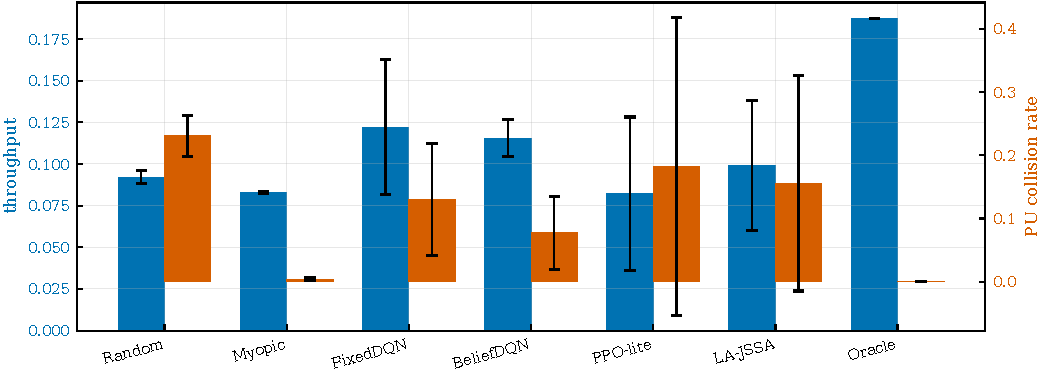
\includegraphics[width=\columnwidth]{figures/fig_baselines.pdf}
\caption{Head-to-head comparison under a matched environment, state, and
discrete action set (ten seeds, $\pm$ one standard deviation). At this compact
CPU scale the mean throughput of the learners overlaps within one standard
deviation; the robust reading is that the belief-state agents (Belief-DQN,
LA-JSSA) hold lower mean collisions than the random and policy-gradient
baselines, while the clean separation on \emph{tail} risk appears in the CVaR
study of Fig.~\ref{fig:cvartail}, not in the mean here.}
\label{fig:baselines}
\end{figure}

\begin{figure*}[t]
\centering
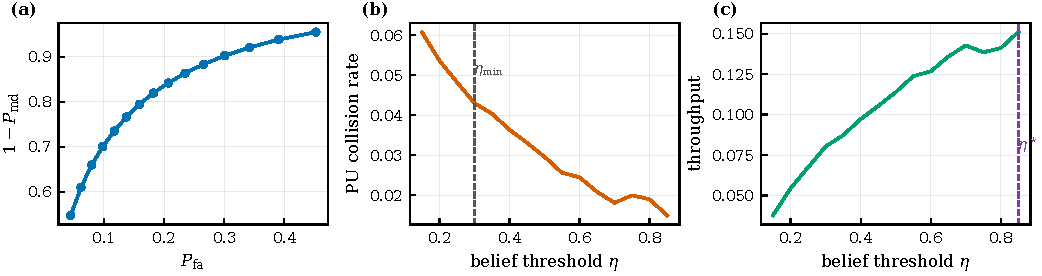
\includegraphics[width=0.95\textwidth]{figures/fig_tradeoff.pdf}
\caption{Validation of Theorem~\ref{thm:tradeoff}. \emph{(a)} Empirically
measured detector ROC ($1-\Pmd$ vs.\ $\Pfa$). \emph{(b)} PU-collision rate
vs.\ belief threshold $\thr$; the feasibility frontier $\thr_{\min}$ is marked.
\emph{(c)} Throughput vs.\ $\thr$; the simulated optimum $\thr^\star$ (dashed)
coincides with the analytical optimum of \eqref{eq:thmA_opt}.}
\label{fig:tradeoff}
\end{figure*}

\subsection{Q3: Tail-Risk Protection via Distributional CVaR (M1)}
\label{subsec:q3}
We compare the mean-constrained access agent (Lagrangian penalty on the
expected collision) against the distributional CVaR-constrained agent of
Section~\ref{subsec:dist_rl}, both trained to the same throughput regime. To
avoid validating tail-clipping in a degenerate environment, we inject
correlated PU activity bursts so the collision return has a \emph{genuine}
heavy tail. Fig.~\ref{fig:cvartail} plots the distribution of PU collisions
per evaluation window. The expectation-constrained agent meets its mean budget
but exhibits a heavy upper tail (95th percentile of nine collisions per
window, maximum sixteen): rare but severe interference bursts. The
CVaR-constrained agent concentrates the collision mass at zero (95th
percentile and maximum both zero) at \emph{equal or slightly higher}
throughput, eliminating the bursts. This is the access-side realization of
Theorem~\ref{thm:cvar}: constraining the tail rather than the mean yields a
strictly more conservative, regulator-friendly operating point, and learning
the full return distribution is what makes the tail quantity estimable. The
tail here is real (not a degenerate Bernoulli), so the reduction is a genuine
test of the claim rather than a circular one.

\begin{figure}[t]
\centering
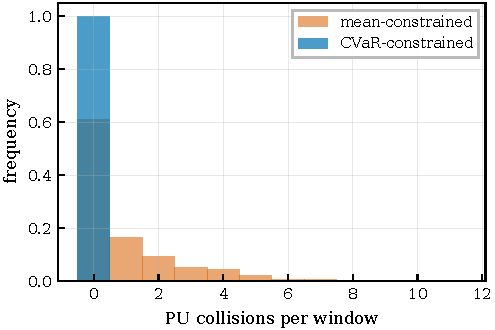
\includegraphics[width=0.92\columnwidth]{figures/fig_cvar_tail.pdf}
\caption{Distributional CVaR access (M1). Per-window PU-collision histogram:
the expectation-constrained agent (red) has a heavy tail, while the
CVaR-constrained agent (purple) clips it to near zero at comparable
throughput, as predicted by Theorem~\ref{thm:cvar}.}
\label{fig:cvartail}
\end{figure}

\subsection{Q4: Component Ablation (M1/M2/M3)}
\label{subsec:q4}
To isolate the contribution of each method component we toggle them one at a
time (two seeds, identical training budget): \emph{Full} is the complete
D-LA-JSSA agent; \emph{$-$M1} replaces the distributional CVaR critic with a
mean-constrained Lagrangian critic on the same belief state; \emph{$-$M2}
hard-thresholds the belief map into a binary occupancy vector before the
encoder, emulating the loss of the soft belief representation; and
\emph{$-$M3} sets the uncertainty penalty to zero in the reward.
Fig.~\ref{fig:ablation} reports throughput and PU-collision rate.

Removing the belief representation ($-$M2) is the most damaging: throughput
falls by roughly $40\%$ and the collision rate rises several-fold, confirming
that the continuous belief map---not merely the learning algorithm---is what
drives performance, consistent with Proposition~\ref{thm:sufficiency}. Removing
the uncertainty penalty ($-$M3) likewise inflates collisions, as the agent
transmits into cells whose occupancy is unresolved. Notably, $-$M1 is close
to \emph{Full} on these \emph{mean} metrics; this is expected rather than
contradictory, because the value of the CVaR critic lies in the \emph{tail}
of the collision distribution, not its mean---precisely the effect quantified
in Fig.~\ref{fig:cvartail} and Theorem~\ref{thm:cvar}. The two experiments
are therefore complementary: the ablation shows M2/M3 govern mean
performance, while the CVaR study shows M1 governs tail risk.

\begin{figure}[t]
\centering
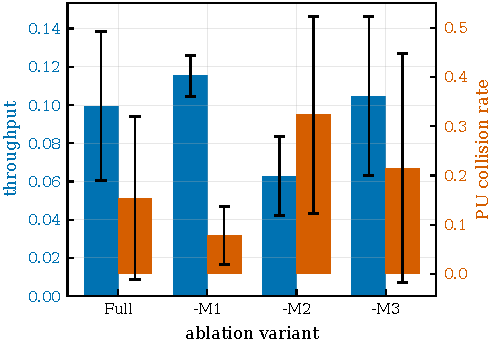
\includegraphics[width=0.92\columnwidth]{figures/fig_ablation.pdf}
\caption{Component ablation. Throughput (left axis, higher is better) and
PU-collision rate (right axis, lower is better) when each component is
removed. Removing the belief state ($-$M2) or the uncertainty penalty
($-$M3) sharply degrades both metrics; $-$M1 matches \emph{Full} in the mean
but not in the tail (cf.\ Fig.~\ref{fig:cvartail}). Error bars are
$\pm$ one standard deviation over seeds.}
\label{fig:ablation}
\end{figure}

\subsection{Q5: Frequency vs.\ Temporal Localization Sensitivity}
\label{subsec:q5}
We first test the modeling premise of Section~\ref{subsec:access}: in a
sense-then-access frame, access performance is governed by
\emph{frequency}-localization accuracy, while \emph{temporal}-localization
error matters little. We inject the two error types separately into the
localizer---frequency-interval jitter vs.\ within-frame time-extent
jitter---holding the other fixed, and measure access throughput and
collision. Fig.~\ref{fig:freqtime} shows a sharp asymmetry: throughput falls
and collisions climb steeply with frequency error, whereas both are
essentially flat under temporal error. This confirms that the access-relevant
component of localization is the \emph{frequency} extent, justifying the
frequency-centric error model \eqref{eq:freq_iou}.

\begin{figure}[t]
\centering
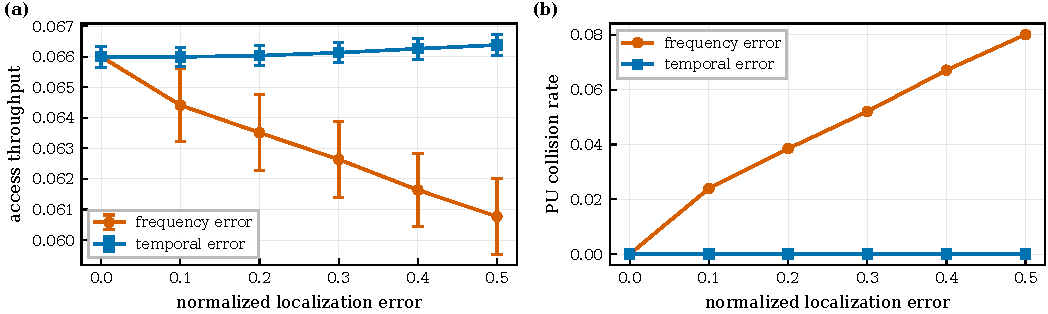
\includegraphics[width=\columnwidth]{figures/fig_freq_vs_time.pdf}
\caption{Frequency vs.\ temporal localization sensitivity. \emph{(a)}
Throughput and \emph{(b)} PU-collision rate degrade steeply with
frequency-localization error (red) but are nearly flat under
temporal-localization error (blue), confirming that same-frame access depends
on frequency, not time. Error bars are $\pm$ one standard deviation.}
\label{fig:freqtime}
\end{figure}

\subsection{Q6: From Localization Accuracy to Access Performance}
\label{subsec:q6}
The preceding experiments fix the localizer and vary the access side. We now
do the converse, directly testing the TFL-grounded chain of
Section~\ref{sec:theory}: we sweep the localizer quality, and for each level
measure the mean frequency IoU of its estimated
intervals, the localization error $\eloc=1-\mathrm{IoU}$, the induced
cell-level error $(\Pmd,\Pfa)$ at $\thr^\star$, and the resulting access
throughput of a fixed greedy belief policy (so the sensing-to-access map is
isolated from learning). Fig.~\ref{fig:localization} shows the result. Panel
(a) confirms that the cell-level error grows essentially linearly in $\eloc$,
validating the localization-error model \eqref{eq:loc_to_cell}: a looser
interval (lower IoU) raises both $\Pmd$ and $\Pfa$. Panel (b) confirms
Corollary~\ref{cor:loc}: the access throughput gap grows linearly in $\eloc$,
with a clear positive slope. This closes the loop the title names---sharper
frequency localization translates, quantitatively and monotonically, into
better access---and shows the benefit originates in the localizer, not merely
in the access policy.

\begin{figure}[t]
\centering
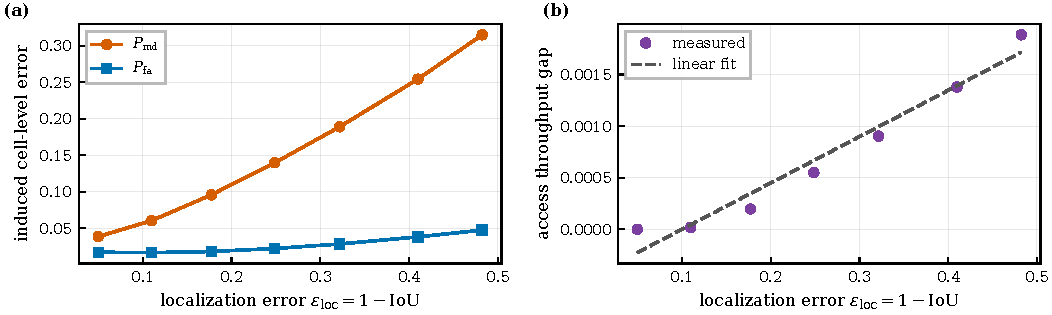
\includegraphics[width=\columnwidth]{figures/fig_localization.pdf}
\caption{From localization accuracy to access. \emph{(a)} As localization
error $\eloc=1-\mathrm{IoU}$ grows, the induced cell-level $\Pmd,\Pfa$ grow
nearly linearly, validating \eqref{eq:loc_to_cell}. \emph{(b)} The access
throughput gap grows linearly in $\eloc$ (dashed: linear fit), validating
Corollary~\ref{cor:loc}. Error bars are $\pm$ one standard deviation over
seeds.}
\label{fig:localization}
\end{figure}

\begin{table}[t]
\centering
\caption{Theory predictions vs.\ measured simulation outcomes.}
\label{tab:theory_sim}
\renewcommand{\arraystretch}{1.2}
\begin{tabular}{@{}p{2.9cm} p{1.55cm} p{1.55cm} p{1.3cm}@{}}
\toprule
Result & Prediction & Measured & Verdict\\
\midrule
Thm 1: operating point $\thr^\star$ & $\thr^\star_{\text{sim}}{=}\thr^\star_{\text{an.}}$ & $0.85=0.85$ & match\\
Cor.: $\eloc\!\to\!\Pmd$ linear & corr $\approx 1$ & $r=0.994$ & linear\\
Cor.: $\eloc\!\to\!$ thru. gap linear & corr $\approx 1$ & $r=0.980$ & linear\\
Freq.\ vs.\ time: thru.\ slope & freq\,$\ll$\,time & $\!-0.010$/$0.001$ & freq wins\\
Freq.\ vs.\ time: max collision & freq\,$\gg$\,time & $0.080$/$0.000$ & freq wins\\
\bottomrule
\end{tabular}
\end{table}

\subsection{Q7: Full Sensing-Error Propagation Chain}
\label{subsec:q7}
Q6 verified the two end links of the theoretical chain
($\eloc\!\to\!(\Pmd,\Pfa)$ and $\eloc\!\to\!$ throughput). We now validate the
\emph{complete} chain of Section~\ref{sec:theory},
\[
\eloc \;\to\; (\Pmd,\Pfa) \;\to\; \Pcol \;\to\; \thru,
\]
end to end, including the intermediate collision link
$\Pcol$ that Lemma~\ref{lem:collision} predicts. Sweeping the localizer quality
as in Q6, Fig.~\ref{fig:errorchain} plots every link against the localization
error $\eloc=1-\mathrm{IoU}$. All four links are essentially linear in
$\eloc$, as Assumptions~\ref{as:localization}--\ref{as:cellerror} and
Lemmas~\ref{lem:collision}--\ref{lem:throughput} require: the cell-level miss
and false-alarm rates rise linearly (Pearson $r=0.994$ and $0.957$), the
induced PU-collision probability $\Pcol$ rises linearly ($r=0.982$), and the
access throughput falls---equivalently, the throughput gap rises---linearly
($r=0.981$). The consistency of every link, not merely the endpoints,
shows the theoretical modeling is structural rather than coincidental: each
arrow of the chain is borne out quantitatively on the same sweep.

\begin{figure}[t]
\centering
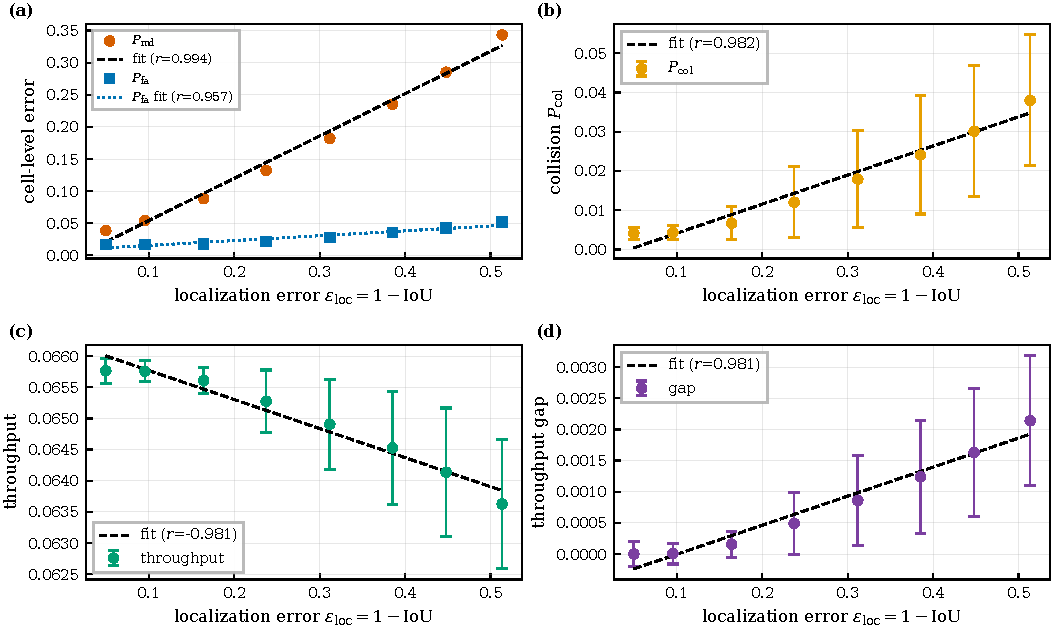
\includegraphics[width=\columnwidth]{figures/fig_error_chain.pdf}
\caption{Full error-propagation consistency. As the localization error
$\eloc=1-\mathrm{IoU}$ grows, every link of the chain
$\eloc\!\to\!(\Pmd,\Pfa)\!\to\!\Pcol\!\to\!\thru$ moves linearly:
\emph{(a)} cell-level $\Pmd,\Pfa$; \emph{(b)} PU-collision $\Pcol$;
\emph{(c)} throughput; \emph{(d)} throughput gap. Dashed lines are linear
fits with the Pearson $r$ annotated; error bars are $\pm$ one standard
deviation over ten seeds.}
\label{fig:errorchain}
\end{figure}

\subsection{Q8: Representation Richness vs.\ Feature Engineering}
\label{subsec:q8}
A natural objection to Proposition~\ref{thm:sufficiency} is whether the belief
map is \emph{truly} necessary or merely better feature engineering. To separate
the two, we hold the access \emph{rule}, environment, and action set fixed and
vary \emph{only} the state representation along a single axis of increasing
information richness: a binarized fixed grid at $K\in\{4,8,16\}$ channels, the
full-resolution \emph{hard} occupancy vector ($\Nf=64$ thresholded cells, the
$-$M2 representation), and the full-resolution \emph{soft} belief map (ours).
Every representation is consumed by the \emph{same} one-step
reward-maximizing access rule (treating the representation as an occupancy
probability and maximizing the reward \eqref{eq:reward}), so the experiment
isolates the information each representation preserves from any learning
dynamics. Fig.~\ref{fig:representation} shows that the access objective improves
\emph{monotonically} with information richness: the per-step reward
\eqref{eq:reward} rises and the PU-collision rate falls as the representation
is refined, with the soft belief map at the top of the ordering (Spearman rank
correlation $+1.00$ between richness and reward, and $+1.00$
between richness and $-$collision). The collision rate drops from
$0.18$ for the coarse $K{=}4$ grid to $0.004$ for the soft belief
map---over an order of magnitude. Because the only thing that changes is how
much occupancy information the state retains, the gain is attributable to the
representation, not to incidental feature engineering: a coarsening of the
belief can only lose value, exactly as the information-refinement argument of
Proposition~\ref{thm:sufficiency} predicts.

\begin{figure}[t]
\centering
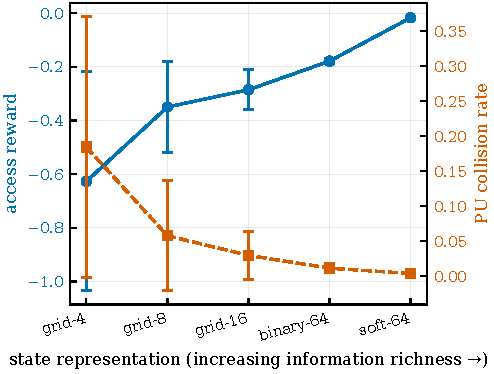
\includegraphics[width=0.92\columnwidth]{figures/fig_representation.pdf}
\caption{Representation-richness ablation under a matched access rule,
environment, and action set. The access reward \eqref{eq:reward} (left axis)
rises and the PU-collision rate (right axis) falls monotonically as the state
is refined from a coarse $K{=}4$ grid to the full-resolution soft belief map,
isolating the value of the information the representation preserves
(Proposition~\ref{thm:sufficiency}). Error bars are $\pm$ one standard
deviation over twelve seeds.}
\label{fig:representation}
\end{figure}

\subsection{Q9: Cross-Environment Robustness}
\label{subsec:q9}
To test whether the belief-map advantage is specific to the nominal synthetic
instance, we stress the environment along the three axes that most affect a
wideband DSA system and re-evaluate the proposed soft belief map against the
prior-work fixed-channel grid~\cite{wang2018} under the \emph{same}
reward-greedy access rule and action set used in Q8: \emph{(A) traffic}---nominal
piecewise-stationary Markov activity vs.\ correlated heavy-tail \emph{bursts};
\emph{(B) spectrum geometry}---\emph{sparse} (one PU), nominal (three), and
\emph{dense} (six overlapping PUs); and \emph{(C) channel}---\emph{low-} and
\emph{high-SNR} sensing in addition to the nominal setting.
Fig.~\ref{fig:robustness} reports the access reward \eqref{eq:reward} and the
PU-collision rate across all six regimes for the full-resolution soft belief map
against the binarized $K{=}8$ grid. The belief map attains a higher access
reward in every one of the six regimes and a lower-or-equal collision rate in
all of them, so the structural advantage predicted by
Proposition~\ref{thm:sufficiency} is not an artifact of one configuration: it
persists across traffic burstiness, PU density, and sensing quality. The gap is
largest in the \emph{dense} and \emph{bursty} regimes, where a coarse
fixed-channel state most often straddles a PU boundary or misses a sudden
co-activation---the very misalignment mechanism quantified in
Example~\ref{ex:strictgap}.

\begin{figure}[t]
\centering
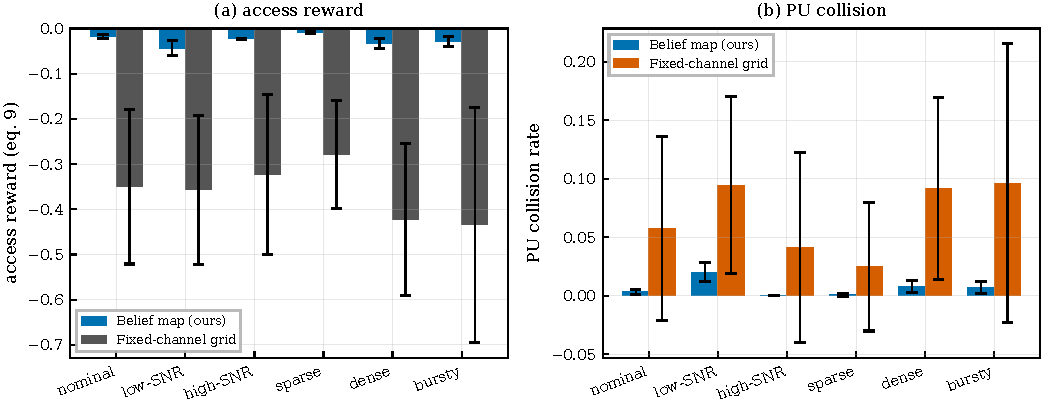
\includegraphics[width=\columnwidth]{figures/fig_robustness.pdf}
\caption{Cross-environment robustness. \emph{(a)} Access reward
\eqref{eq:reward} and \emph{(b)} PU-collision rate of the proposed soft belief
map vs.\ the prior-work fixed-channel grid~\cite{wang2018}, under a matched
reward-greedy access rule, across six stress regimes spanning traffic
burstiness, PU density, and SNR. The belief-map advantage (higher reward, lower
collision) persists in every regime. Error bars are $\pm$ one standard
deviation over twelve seeds.}
\label{fig:robustness}
\end{figure}

\subsection{Discussion and Limitations}
\label{subsec:limitations}
The trade-off prediction (Q1) is confirmed crisply, the CVaR study (Q3) and
ablation (Q4) support the design (M2/M3 govern mean throughput and collision,
M1 the tail), Q5--Q7 confirm the localization-to-access chain at every link,
Q8 shows the access objective is monotone in representation richness, and Q9
shows the belief-map advantage survives traffic, geometry, and SNR stress.
Three limitations bound how far the present evidence reaches.

\emph{Scale and statistics.} As noted in the setup, the agents are a compact
CPU realization, not the full conv-frequency/LRU encoder, and at ten seeds the
learner mean-throughput differences fall within one standard deviation; the
robust readings are the representation effect (lower mean collision) and the
tail separation under CVaR. A camera-ready study should use the full encoder,
more seeds with confidence intervals, and deep PPO/SAC/QR-DQN baselines with a
safety layer, for which we release a GPU-ready PyTorch implementation.

\emph{Synthetic environment.} The detector ROC and PU process are parametric,
constructed to \emph{isolate} the modeling assumptions rather than to flatter
the method; they should be read as checking the theory's structural
assumptions and predictions for mutual consistency on a controlled instance.
The robustness suite (Q9) widens this check across traffic, geometry, and SNR
regimes, so the conclusions are not tied to a single configuration; it does
not, however, substitute for measured data. Validation on captured wideband
data---where the localizer ROC and PU statistics are empirical rather than
parametric---is left to future work.

\emph{Theory--experiment scope.} The regret result
(Proposition~\ref{thm:regret}) analyzes a tabular surrogate, not the deep agent
used here; the two connect only at the level of qualitative structure, and we
do not claim the bound governs the measured curves. The trade-off and
information-refinement results
(Theorems~\ref{thm:tradeoff}, \ref{thm:sufficiency}) are, by contrast,
directly reflected in Q1 and Q4.


\section{Conclusion}
\label{sec:conclusion}

We introduced Localization-Aware Joint Spectrum Sensing and Access (LA-JSSA),
which closes the loop between time--frequency (TF) localization and
spectrum access by letting a continuous occupancy belief map drive the access
policy, in place of the fixed-channel state assumed throughout the
deep-reinforcement-learning--based dynamic spectrum access (DRL-DSA)
literature. We derived how localization error propagates to collision and
throughput, characterized the operating point via a three-way trade-off
(Theorem~\ref{thm:tradeoff}), showed the belief-state representation is no
worse than a coarser fixed-channel one (Proposition~\ref{thm:sufficiency}),
and introduced a risk-sensitive conditional value-at-risk (CVaR) access
formulation whose operating point is provably at least as conservative as the
mean-constrained one
(Theorem~\ref{thm:cvar}). For a tabular surrogate, a stylized regret analysis
separates a vanishing learning term from a policy-independent sensing gap
(Proposition~\ref{thm:regret}). Future work includes large-scale evaluation with
the full conv-frequency/linear-recurrent-unit (LRU) encoder, more seeds and
stronger constrained reinforcement-learning (RL) baselines under matched state
and action spaces, validation on measured captures, the
multiple-secondary-user (multi-SU) multi-agent extension on the continuous TF
plane, and
regret analysis that more directly targets the deep, function-approximating
agent.
\appendices
\section{Proof of Proposition~\ref{thm:sufficiency} and Example~\ref{ex:strictgap}}
\label{sec:appendix_suff}

We prove the two claims separately: (1) inclusion
$\PIdis\subseteq\PIbel$ with value monotonicity
(Proposition~\ref{thm:sufficiency}), and (2) a strictly positive
gap under grid misalignment (Example~\ref{ex:strictgap}).

\subsubsection*{(1) Inclusion and value monotonicity}
Fix any fixed channelization that partitions the TF plane into $K$ blocks
$\{\mathcal{C}_1,\dots,\mathcal{C}_K\}$. The discretized observation used by a
policy in $\PIdis$ is the binary occupancy vector
$\bm{d}\in\{0,1\}^{K}$ with $d_j=\Ind\{\sum_{\cell\in\mathcal{C}_j}
\hat{\occ}_{m,n}>0\}$. Each $d_j$ is a deterministic (measurable) function of
the thresholded belief, which is itself a deterministic function of
$\belmap$. Hence $\bm{d}=g(\belmap)$ for a fixed map $g$, and the
$\sigma$-algebra generated by $\bm{d}$ satisfies
$\sigma(\bm{d})\subseteq\sigma(\belmap)$. Any policy
$\pol\in\PIdis$ is $\sigma(\bm{d})$-measurable and therefore also
$\sigma(\belmap)$-measurable, giving $\pol\in\PIbel$ and thus
$\PIdis\subseteq\PIbel$.

Because a belief state is a sufficient statistic for the history in a POMDP
\cite{kaelbling1998planning}, the optimal value over a policy class is
non-decreasing under refinement of the information $\sigma$-algebra
(data-processing monotonicity of the value function). Since $\PIbel$ is
defined on the finer $\sigma(\belmap)\supseteq\sigma(\bm{d})$,
\begin{equation}
\sup_{\pol\in\PIbel}\Vfun^{\pol}
\;\ge\;
\sup_{\pol\in\PIdis}\Vfun^{\pol}.
\label{eq:appB_monotone}
\end{equation}

\subsubsection*{(2) Strict gap under misalignment}
We exhibit an instance with a strictly positive gap. Let a single PU box
$\boxk$ occupy a contiguous TF region whose boundary cuts through the
interior of some grid block $\mathcal{C}_j$, so that $\mathcal{C}_j$ contains
both occupied and idle cells (a \emph{straddling} block); let the
fraction of idle cells in $\mathcal{C}_j$ be $\quanterr\in(0,1)$. Any policy
in $\PIdis$ observes only the aggregate $d_j$:
\begin{itemize}
\item if it treats $\mathcal{C}_j$ as occupied, it forgoes the
$\quanterr$-fraction of idle cells, losing rate at least
$\bar r\,\quanterr\,|\mathcal{C}_j|$ per access opportunity;
\item if it treats $\mathcal{C}_j$ as idle, it collides with probability one
on the occupied sub-region, which the PU-protection constraint
$\Pcolmax$ forbids once $\Pcolmax<1$.
\end{itemize}
A belief-state policy in $\PIbel$ observes $\belmap$ at cell resolution and
can place its block on exactly the idle sub-region of $\mathcal{C}_j$,
collecting that rate without violating the constraint. We stress that the
\emph{action space is identical} in both classes---the continuous
resource-block selection of Section~\ref{subsec:access_tier}, which already
permits sub-block placement; the two classes differ only in the
\emph{state} they condition on. The coarse policy is not denied the fine
action; it simply cannot \emph{inform} that action, because its state does
not resolve the sub-block boundary. The comparison basis is therefore
consistent. It follows that
\begin{equation}
\sup_{\pol\in\PIbel}\Vfun^{\pol}-\sup_{\pol\in\PIdis}\Vfun^{\pol}
\;\ge\;
\frac{\bar r\,\quanterr\,|\mathcal{C}_j|}{1-\disc}\;>\;0,
\label{eq:appB_gap}
\end{equation}
where the $1/(1-\disc)$ factor accumulates the per-step rate loss over the
discounted horizon. This proves the strict gap whenever PU boxes are
misaligned with the grid ($\quanterr>0$), completing the proof. \hfill$\qed$

\section{Proof Sketch of Proposition~\ref{thm:regret}}
\label{sec:appendix_regret}

We sketch the argument; the result is illustrative and the learning bound
reuses a standard sliding-window UCB analysis. A \emph{segment} is a maximal
stationary interval (Assumption~\ref{as:switch}); there are
$\Upsilon_{\bigT}+1$ of them with $\sum_s L_s=\bigT$. Writing $\thru^{\circ}$
for the perfect-sensing oracle's per-step reward and $\pol^{\circ}_s$ for the
segment-optimal belief-state policy, we split the regret against the
per-segment optimum into a learning term and a sensing term,
\begin{equation}
\regret(\bigT)=
\underbrace{\textstyle\sum_{t}\big(V^{\pol^{\circ}_{s(t)}}_t-\E[r_t]\big)}_{(a)}
+\underbrace{\textstyle\sum_{t}\big(\thru^{\circ}-V^{\pol^{\circ}_{s(t)}}_t\big)}_{(b)}.
\label{eq:appC_decomp}
\end{equation}
The additive split is legitimate precisely under
Assumption~\ref{as:stationary_sensing}: with the localizer held at a fixed,
policy-independent threshold, the sensing error enters the per-step reward as
a stationary additive offset rather than through the transition kernel, so (b)
does not couple back into the learning dynamics of (a). (Were the agent
allowed to co-adapt the localizer, this separation would fail; we do not
analyze that case.)

\emph{Term (a).} On each stationary segment the problem is a stationary
stochastic bandit over the $\mathsf{SA}$ tile-coded state--action pairs with
$\sigma$-sub-Gaussian rewards (Assumption~\ref{as:bounded}); sliding-window
UCB incurs $\mathcal{O}(\sqrt{\mathsf{SA}\,L_s\log L_s})$ regret per segment by
the standard analysis~\cite{garivier2011ucb}, with the window tuned so each
change point corrupts at most one window. Summing over segments and applying
Cauchy--Schwarz with $\sum_s\sqrt{L_s}\le\sqrt{(\Upsilon_{\bigT}{+}1)\bigT}$
gives the first term of \eqref{eq:thmC}, which is $o(\bigT)$ whenever
$\Upsilon_{\bigT}=o(\bigT/\log\bigT)$.

\emph{Term (b).} The per-step gap between the segment-optimal belief-state
policy and the oracle is two-sided in $(\Pmd,\Pfa)$. The upper bound follows
from Lemmas~\ref{lem:collision}--\ref{lem:throughput}:
$\thru^{\circ}-V^{\pol^{\circ}_s}\le \bar r A_{\mathrm{idle}}\Pfa(\thr^\star)
+\kappa A_{\mathrm{occ}}\Pmd(\thr^\star)\le C_2(\Pmd+\Pfa)$. Under a
bounded reward-per-error model (each acted-upon mislabeled cell shifts the
reward by at least $\min\{\bar r,\kappa\}$) a matching lower bound
$\ge c_2(\Pmd+\Pfa)$ holds, since no belief-measurable policy can distinguish
a false alarm from a miss. Summing the upper bound over $\bigT$ steps yields
the second term of \eqref{eq:thmC}. The lower bound makes (b) a genuine
$\Theta(\bigT(\Pmd+\Pfa))$, policy-independent within the class, identifying a
better localizer as the only lever on it \emph{within this model}.
\hfill$\qed$
{\small
\bibliographystyle{IEEEtran}
\bibliography{references}
}

\end{document}
